%%%%%%%%%%%%%%%%%%%%%%%%%%%%%%%%%%%%%%%%%%%%%%%%%%%%%%%%%
%%   $RCSfile: hpsg04.tex,v $
%%  $Revision: 1.1 $
%%      $Date: 2004/08/11 09:53:01 $
%%     Author: Stefan Mueller (CL Uni Bremen)
%%    Purpose: 
%%   Language: LaTeX
%%%%%%%%%%%%%%%%%%%%%%%%%%%%%%%%%%%%%%%%%%%%%%%%%%%%%%%%%
%%
%% $Log: hpsg04.tex,v $
%% Revision 1.1  2004/08/11 09:53:01  stefan
%% *** empty log message ***
%%
%% Revision 1.1  2003/10/12 13:42:57  stefan
%% Initial revision
%%
%%%%%%%%%%%%%%%%%%%%%%%%%%%%%%%%%%%%%%%%%%%%%%%%%%%%%%%%%

\documentclass[11pt,a4paper,fleqn]{article}
\usepackage{times}
\thispagestyle{empty}



\usepackage[T1]{fontenc}   % Silbentrennung

\usepackage[latin1,utf8x]{inputenc}

\usepackage[bookmarks=true,bookmarksopen=true,%
breaklinks=true,%
draft=false,colorlinks=false,plainpages=false,hyperfootnotes=false,%
linkcolor=black,%
pagecolor=black,%
pdfauthor={Stefan Müller (Editor)},%
pdftitle={Proceedings of the HPSG 2010 Conference},%
pdfkeywords={HPSG}%,
pdftex=true%
%ps2pdf=true  %ohne diesen Treiber geht der Zeilenumbruch in URLs
]{hyperref}% for pdf files

\usepackage{pdfpages}


\hypersetup{colorlinks=false, pdfborder={0 0 0}}

\begin{document}

\begin{center}
{\Large
                Proceedings of the HPSG 2011 Conference\\[\baselineskip]

                       Department of Linguistics, University of Washington\\[\baselineskip]

                        Stefan M{\"u}ller (Editor)\\[\baselineskip]

                                2011\\[\baselineskip]

                          CSLI Publications\\[\baselineskip]

              http://csli-publications.stanford.edu/ 
}
\end{center}
\newpage
\tableofcontents

\newpage

\section{Editor's Note}

The 18th International Conference on Head-Driven Phrase Structure Grammar (2011) was held at the University of Washington.

The conference featured 2 invited talks and 16 papers, and 1 poster selected by the program committee (Anne Abeillé,
Doug Arnold,
Emily M. Bender,
Philippe Blache,
Olivier Bonami,
Robert Borsley,
Gosse Bouma,
Rui Chaves,
Berthold Crysmann (chair),
Dan Flickinger,
Danièle Godard,
Lars Hellan,
Anke Holler,
Jong-Bok Kim,
Jean-Pierre Koenig,
Valia Kordoni,
Anna Kupsc,
Robert Levine,
Rob Malouf,
Nurit Melnik,
Philip Miller,
Stefan Müller,
Gerald Penn,
Adam Przepiorkowski,
Frank Richter,
Ivan Sag,
Manfred Sailer,
Jesse Tseng,
Frank Van Eynde,
Gert Webelhuth,
Stephen Wechsler,
Shuichi Yatabe).

A workshop about \emph{Information Structure and Formal Grammar}
was attached to the conference. It featured one invited talk and 8 papers and a poster, selected by the program
committee of this workshop (Felix Bildhauer,
Daniel Büring,
Berthold Crysmann (chair),
Kordula De Kuthy,
Elisabet Engdahl,
Claire Gardent,
Jonathan Ginzburg,
Tracy Holloway King,
Manfred Krifka,
Jean-Marie Marandin,
Laura Michaelis,
Stefan Müller,
Irina Nikolaeva,
Patrizia Paggio,
Arndt Riester,
Mats Rooth,
Mark Steedman,
Malte Zimmermann).

% wie viele?
%In total there were 29  submissions to the conference and 24 submissions to the workshop.
We want to thank the respective program committees for putting this nice program together.



Thanks go to Emily M. Bender (chair), Joshua Crowgey,
Michael Goodman,
Varya Gracheva,
Prescott Klassen,
Naoko Komoto,
Clarissa Surek-Clark,
Emily Silgard,
Sanghoun Song,
Lisa Tittle, and David Wax, who were in charge of local arrangements.


As in the past years the contributions to the conference proceedings are based on the five page abstract
that was reviewed by the respective program committees, but there is no additional reviewing of the
longer contribution to the proceedings.
To ensure easy access and fast publication we have chosen an electronic format.


The proceedings include all the papers except those by Olivier Bonami, Rui Chaves, Anna Gazdik,
Tibor Kiss, Mats Rooth, and Thomas Wasow and David Clausen.



\newpage
\part{Contributions to the Main Conference}


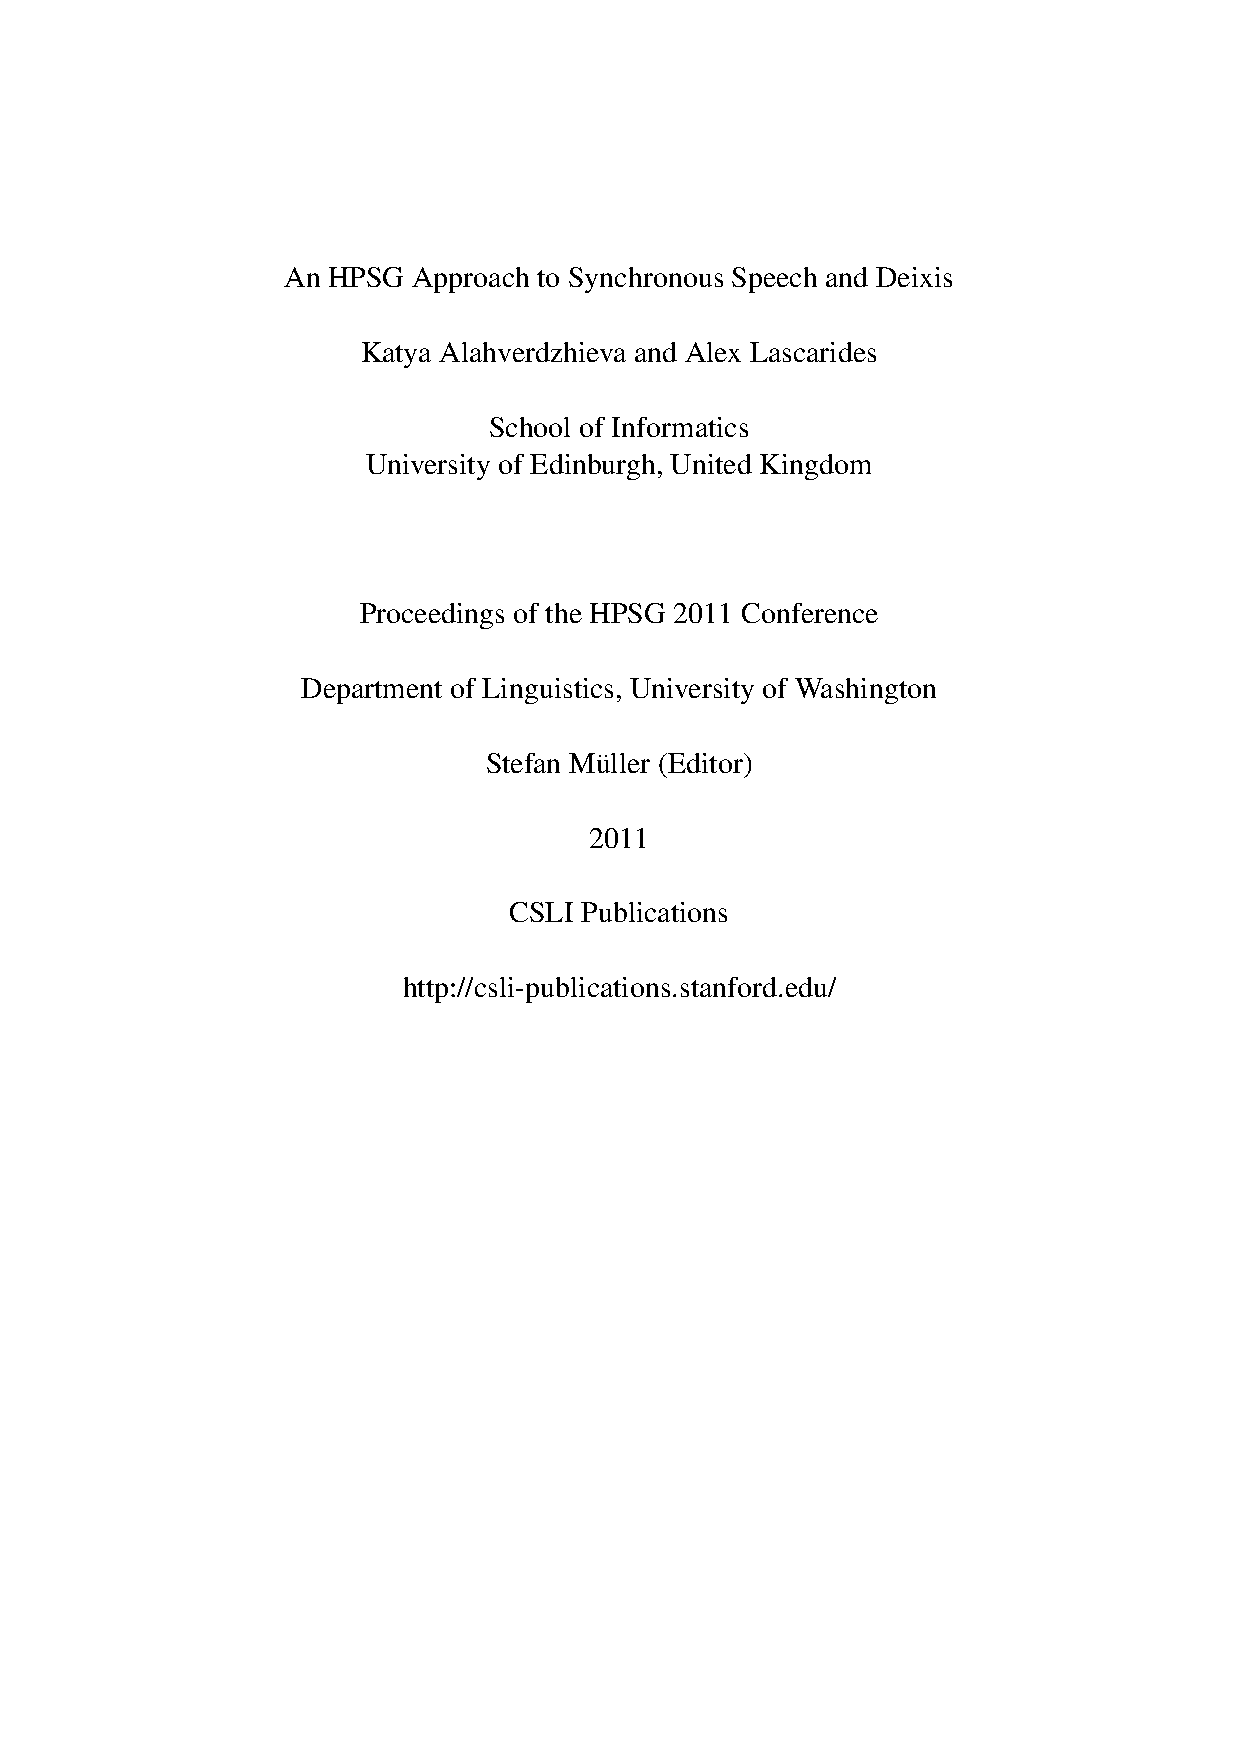
\includepdf[pages=-,pagecommand=\thispagestyle{plain},
            addtotoc={1,section,1,
            {Katya Alahverdzhieva and Alex Lascarides: An HPSG Approach to Synchronous Speech and Deixis},
             al}]{alahverdzhieva-lascarides.pdf}


\includepdf[pages=-,pagecommand=\thispagestyle{plain},
            addtotoc={1,section,1,
            {Douglas Ball: Morphology in the ‘Wrong’ Place: The Curious Case of Coast Tsimshian Connectives},
             ball}]{ball.pdf}

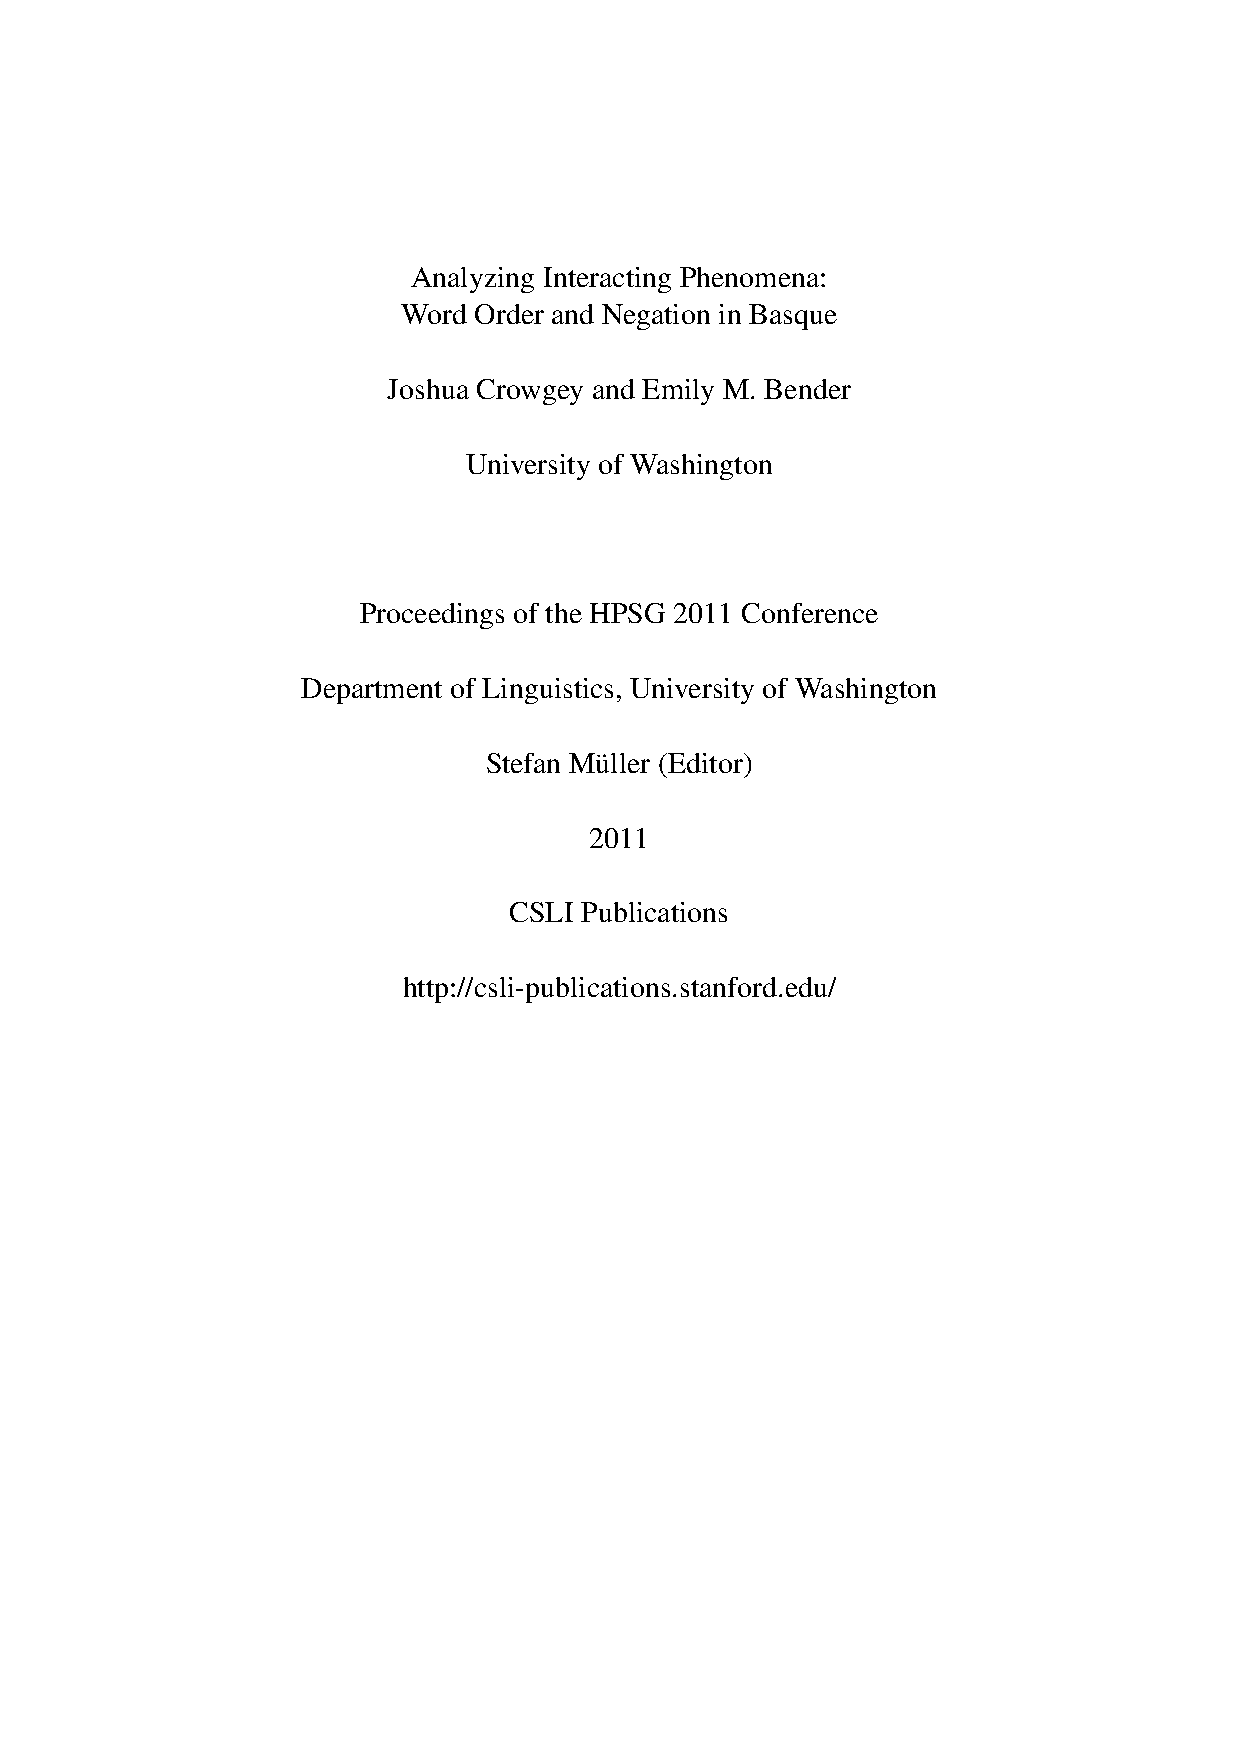
\includepdf[pages=-,pagecommand=\thispagestyle{plain},
            addtotoc={1,section,1,
            {Joshua Crowgey and Emily M. Bender: Analyzing Interacting Phenomena: Word Order and Negation in Basque},
             cb}]{crowgey-bender.pdf}


\includepdf[pages=-,pagecommand=\thispagestyle{plain},
            addtotoc={1,section,1,
            {Michael Hahn: Null Conjuncts and Bound Pronouns in Arabic},
             hahn}]{hahn.pdf}

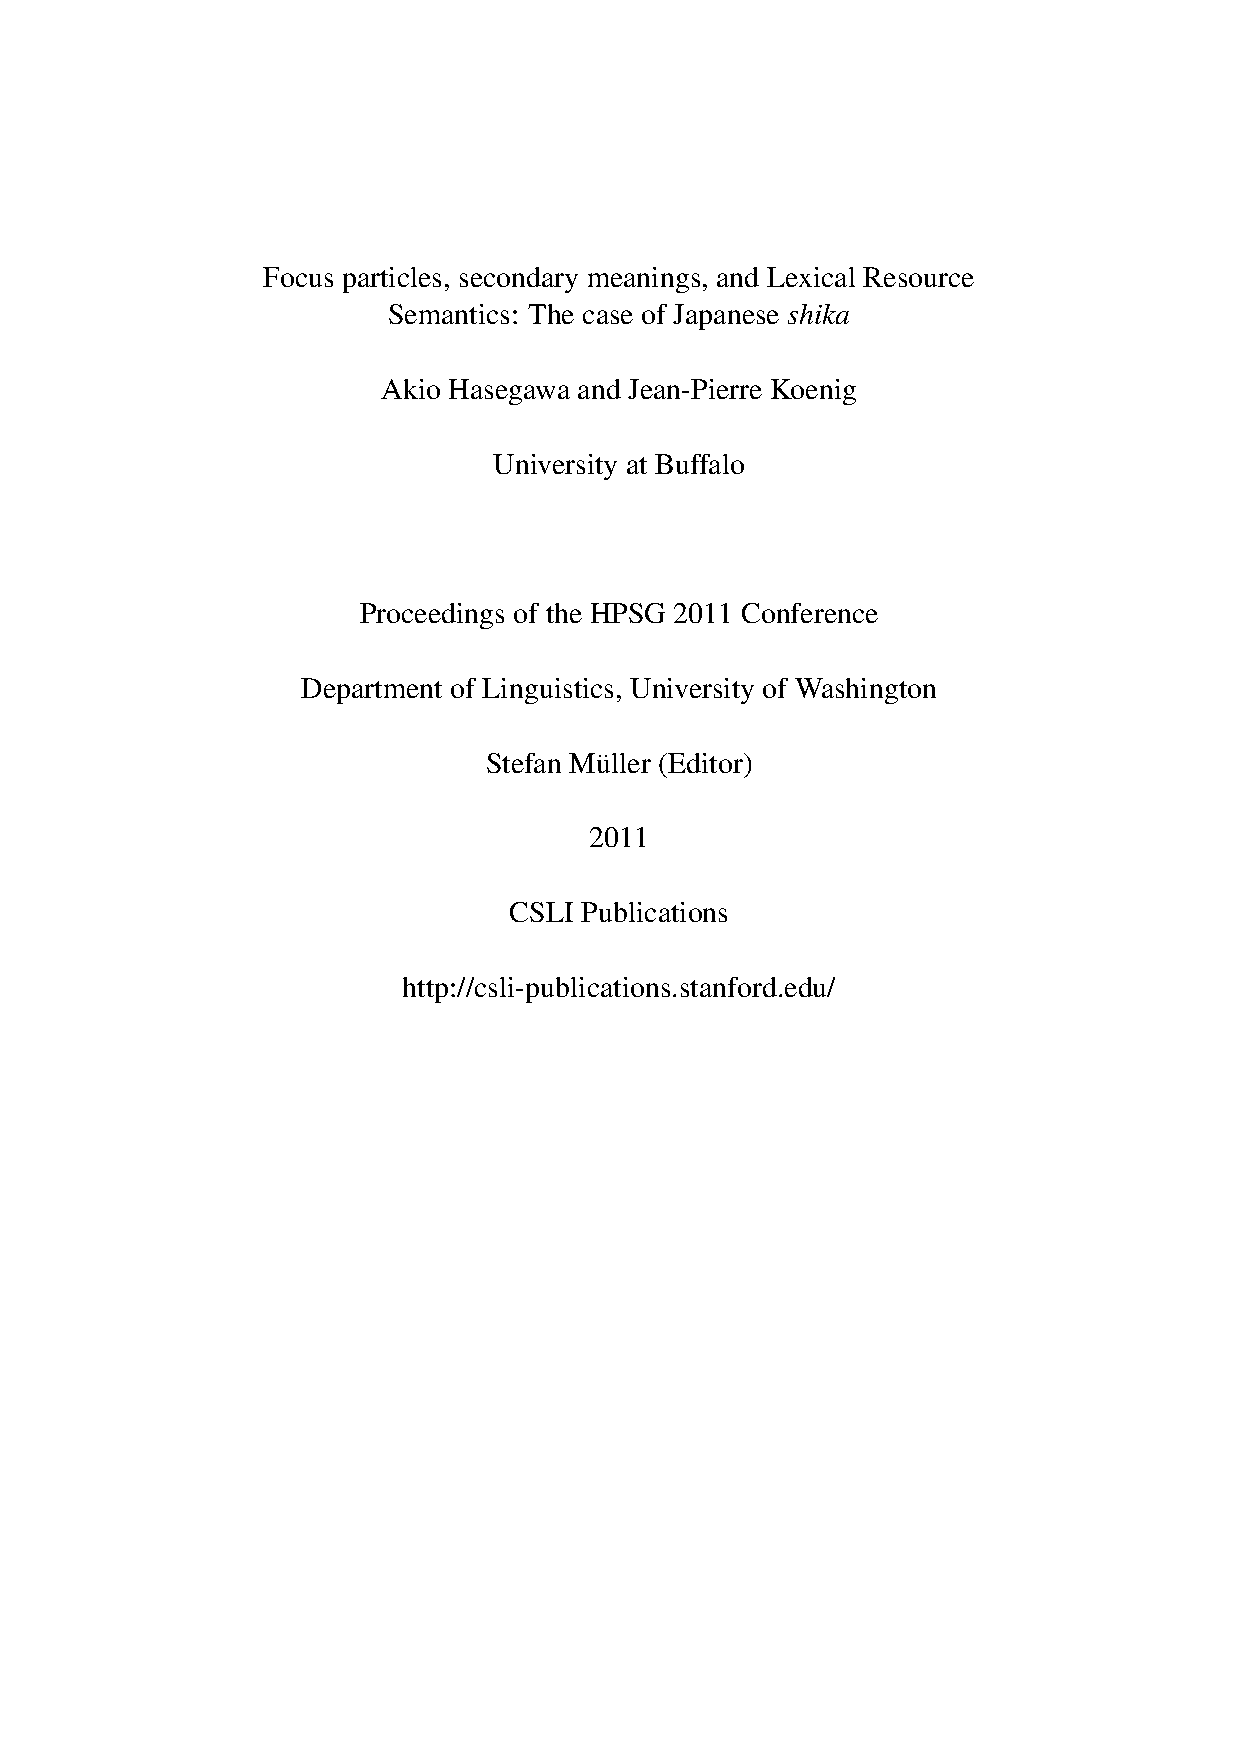
\includepdf[pages=-,pagecommand=\thispagestyle{plain},
            addtotoc={1,section,1,
            {Akio Hasegawa and Jean-Pierre Koenig: Focus particles, secondary meanings, and Lexical Resource Semantics: The case of Japanese \emph{shika}},
             hk}]{hasegawa-koenig.pdf}

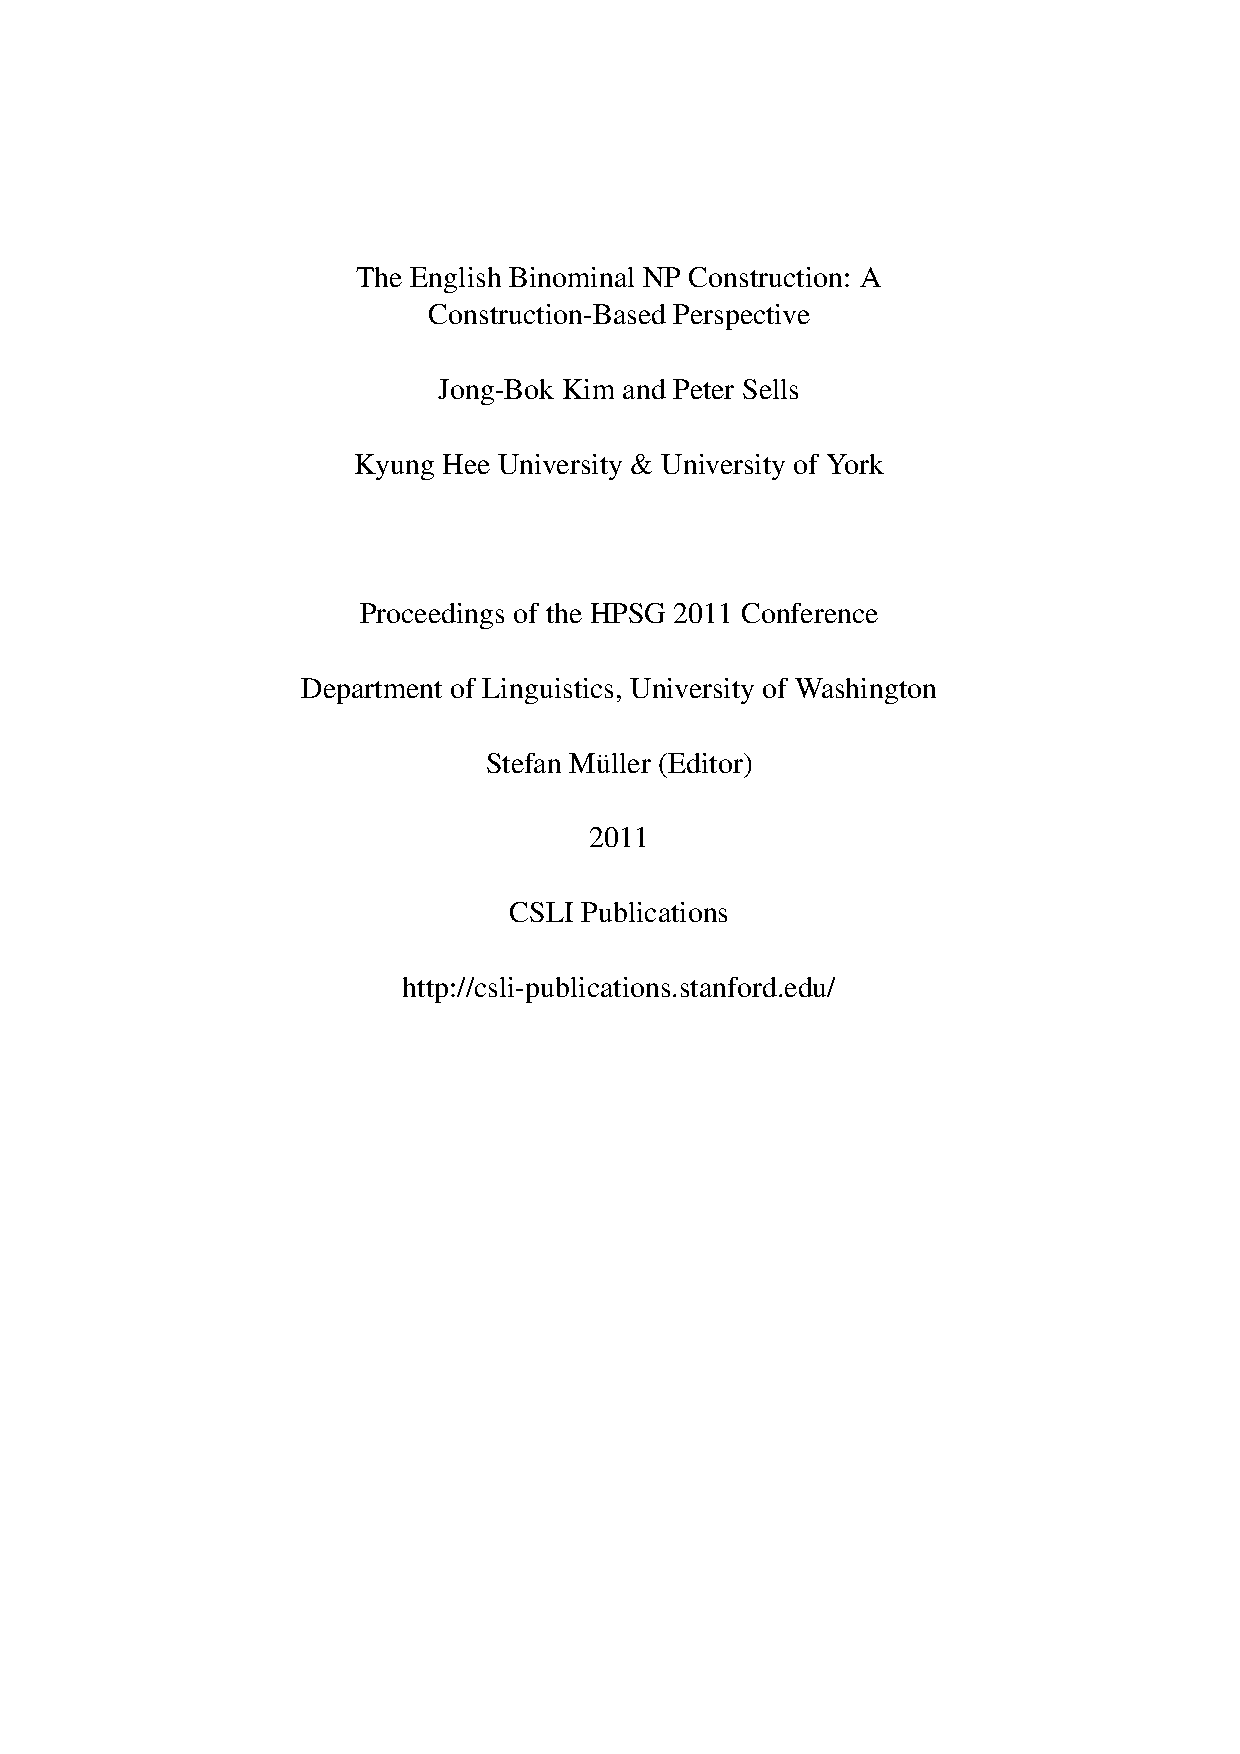
\includepdf[pages=-,pagecommand=\thispagestyle{plain},
            addtotoc={1,section,1,
            {Jong-Bok Kim and Peter Sells: The English Binominal NP Construction: A Construction-Based Perspective},
             ks}]{kim-sells.pdf}

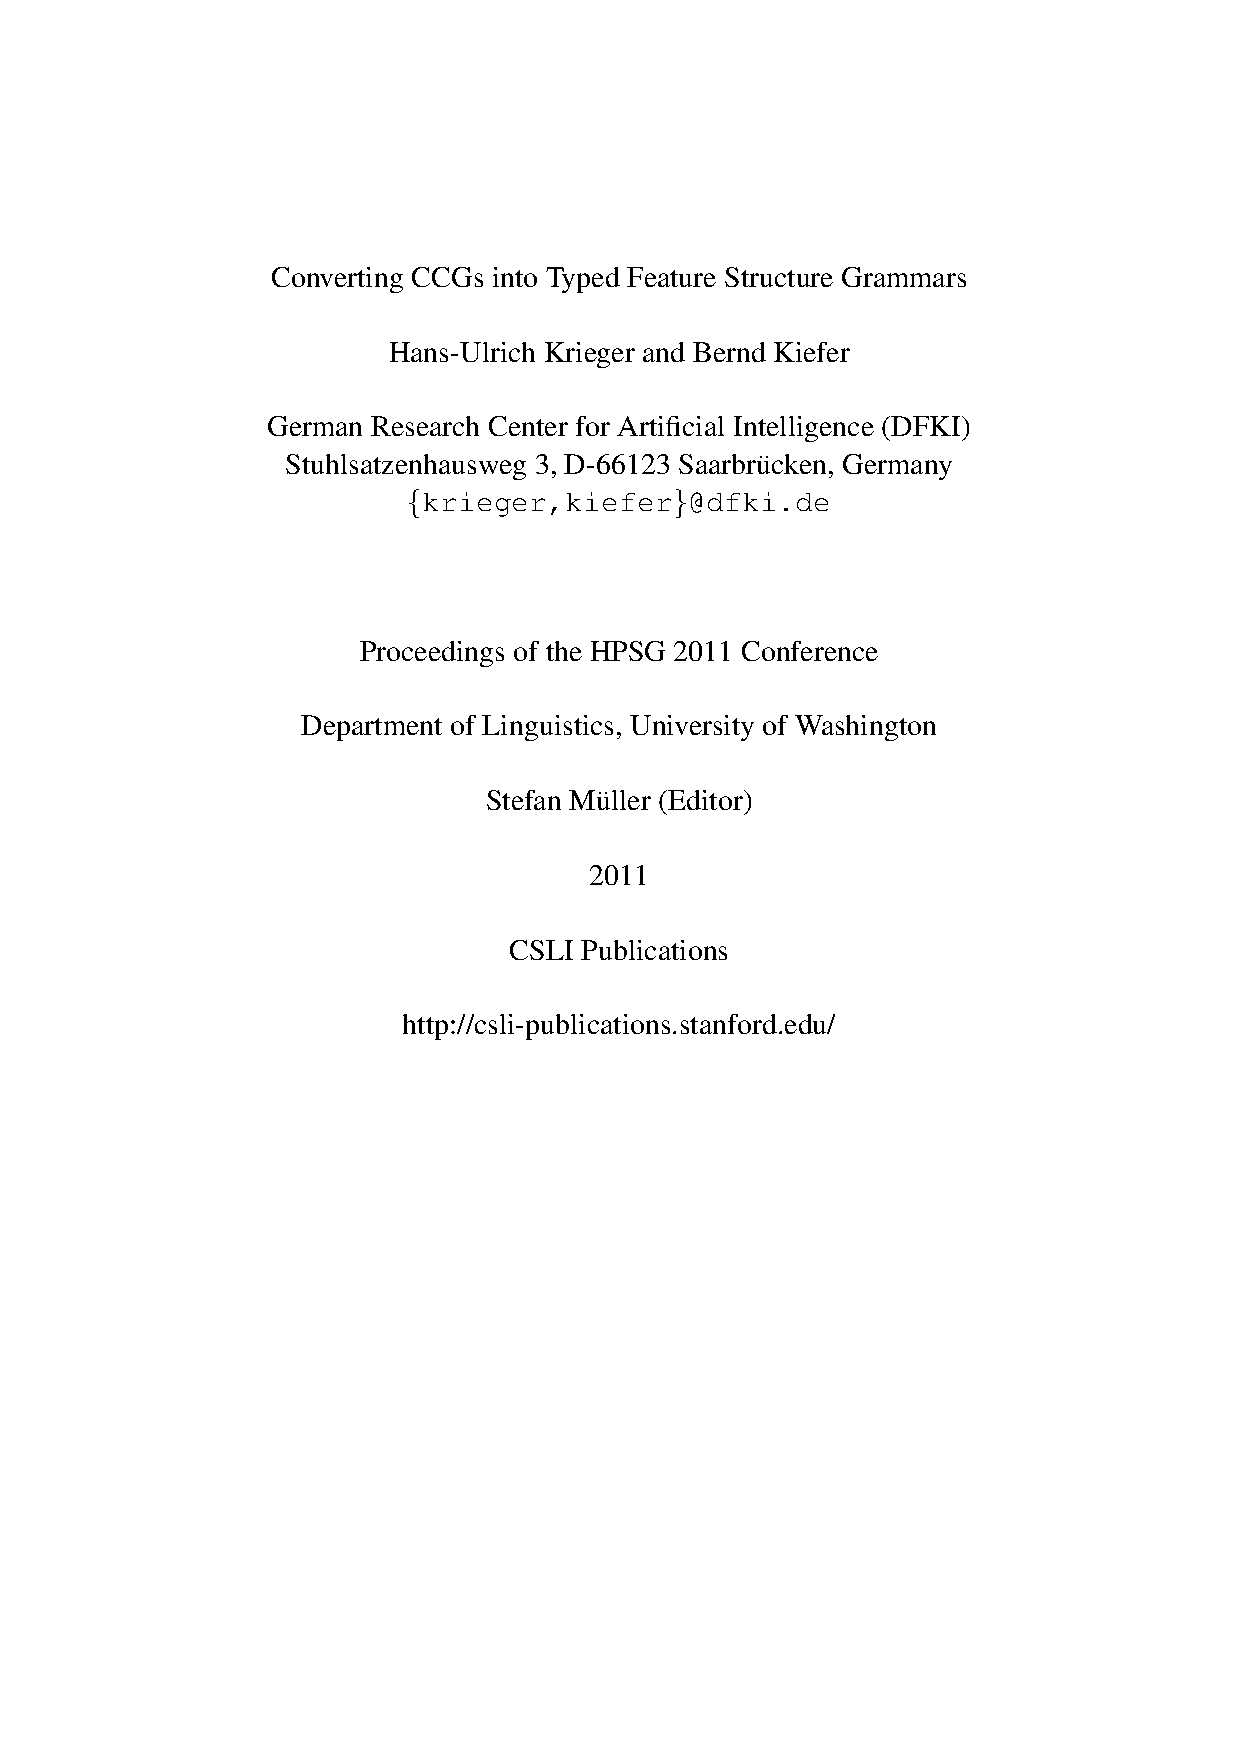
\includepdf[pages=-,pagecommand=\thispagestyle{plain},
            addtotoc={1,section,1,
            {Hans-Ulrich Krieger and Bernd Kiefer: Converting CCGs into Typed Feature Structure Grammars},
             kk}]{krieger-kiefer.pdf}


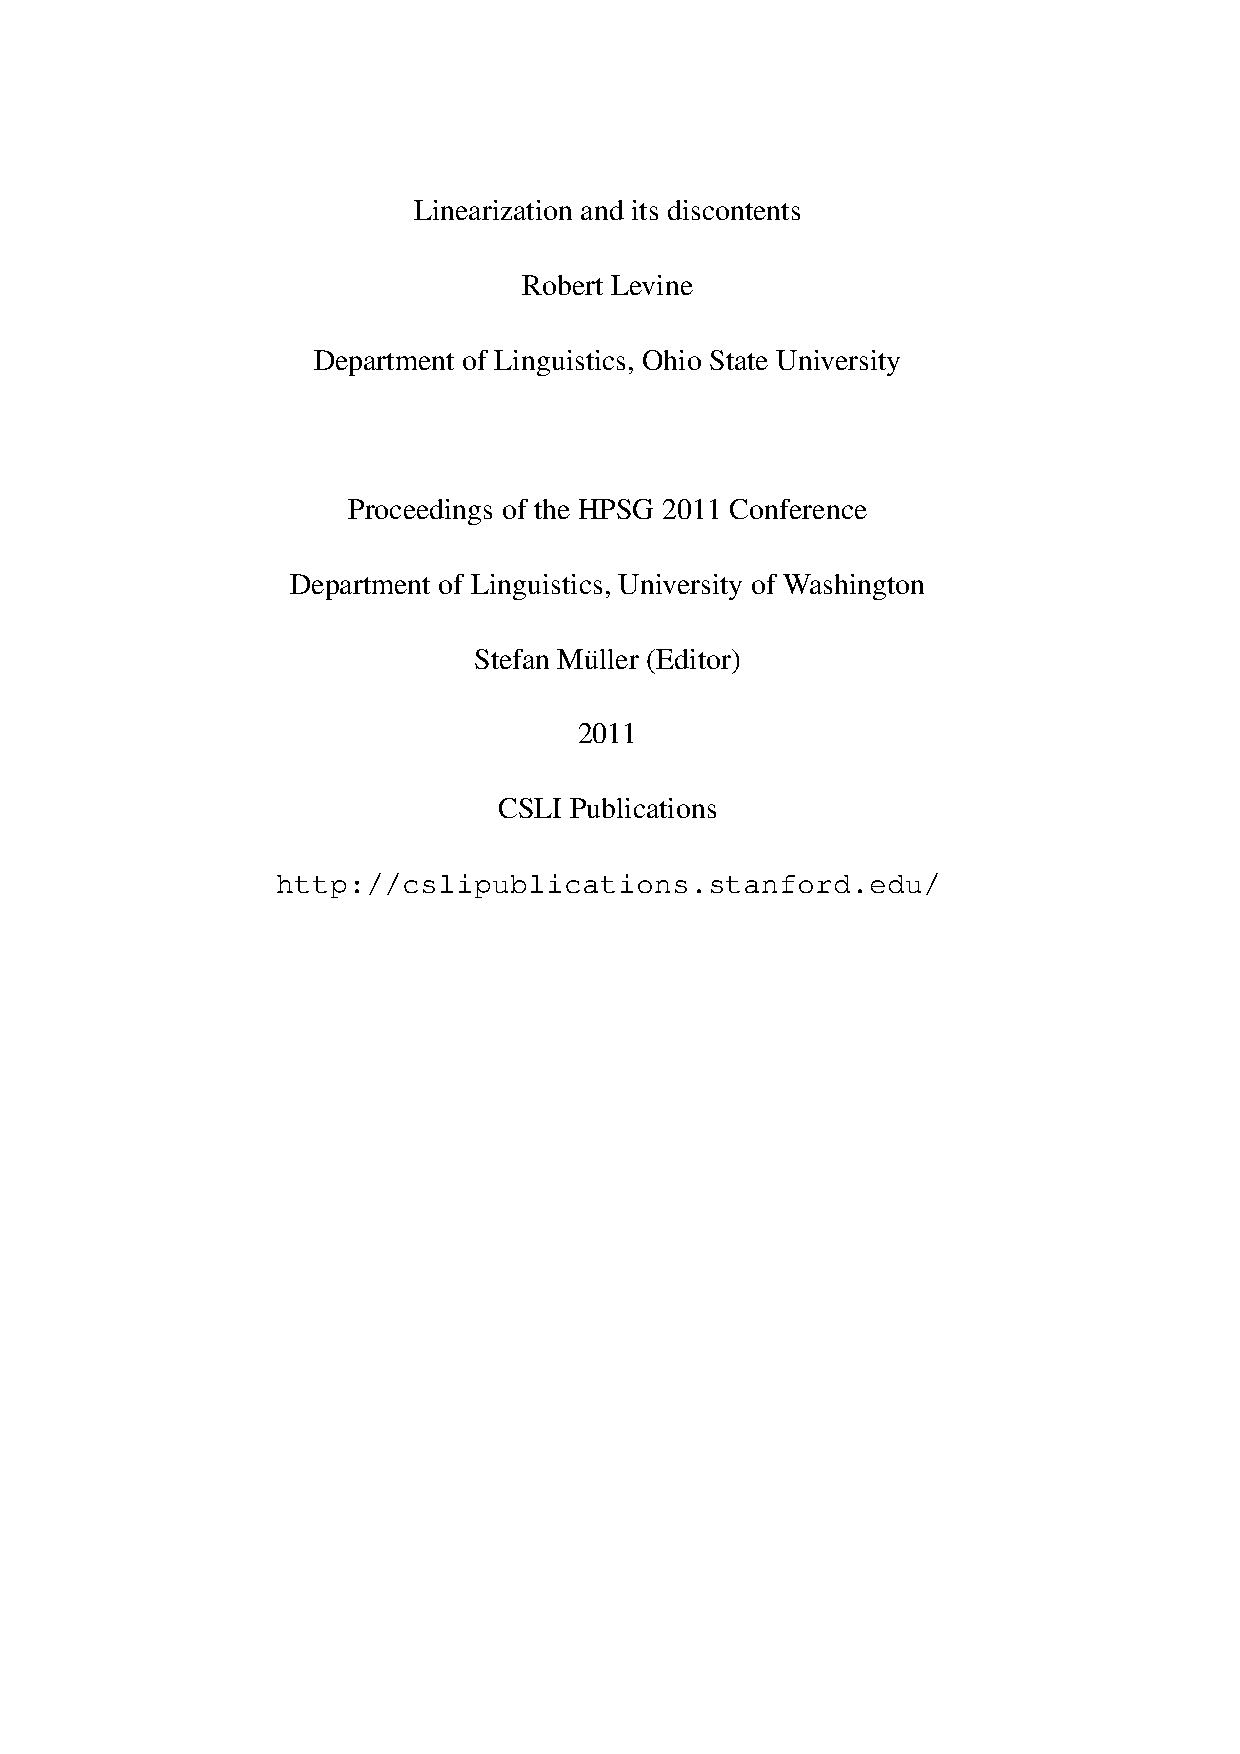
\includepdf[pages=-,pagecommand=\thispagestyle{plain},
            addtotoc={1,section,1,
            {Robert Levine: Linearization and its discontents},
             levine}]{levine.pdf}

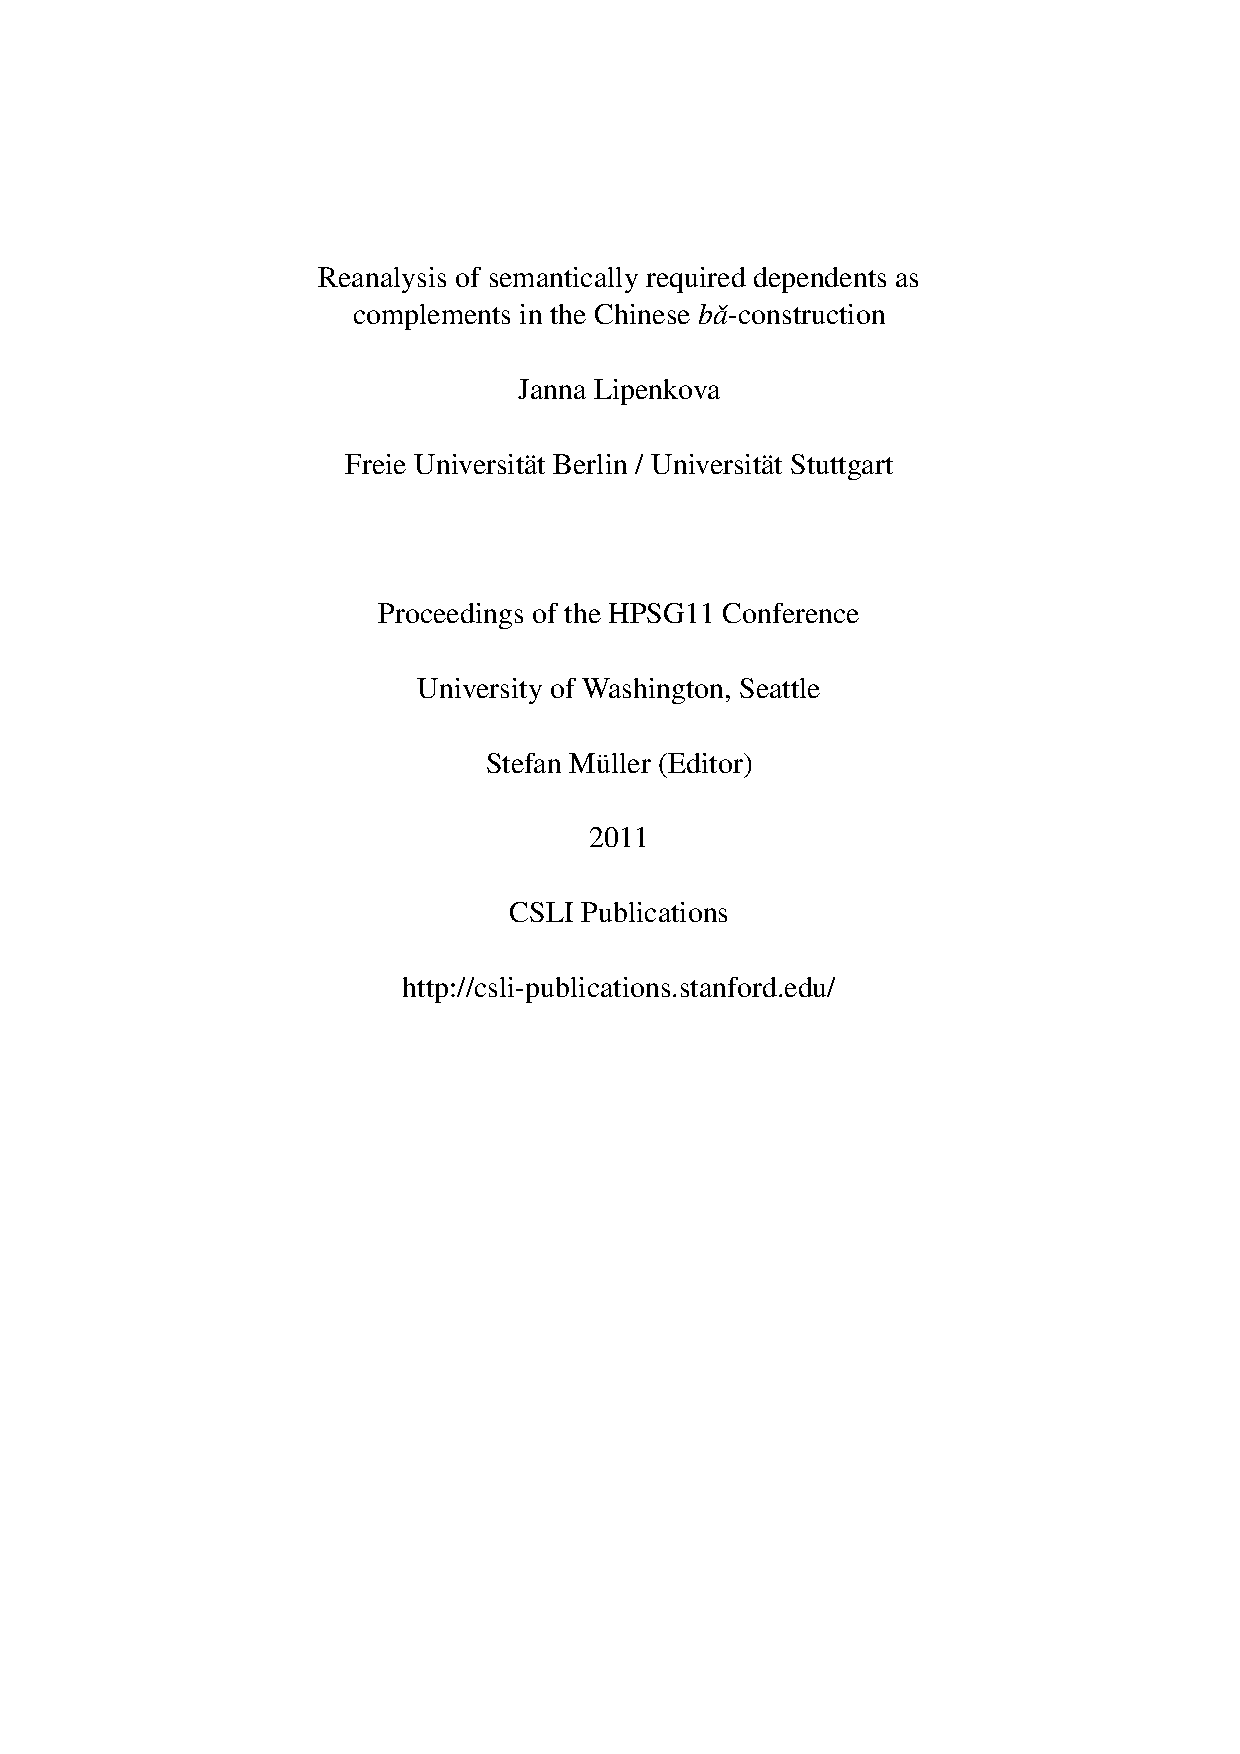
\includepdf[pages=-,pagecommand=\thispagestyle{plain},
            addtotoc={1,section,1,
            {Janna Lipenkova: Reanalysis of semantically required dependents as complements in the Chinese \emph{ba}-construction},
             lipenkova}]{lipenkova.pdf}


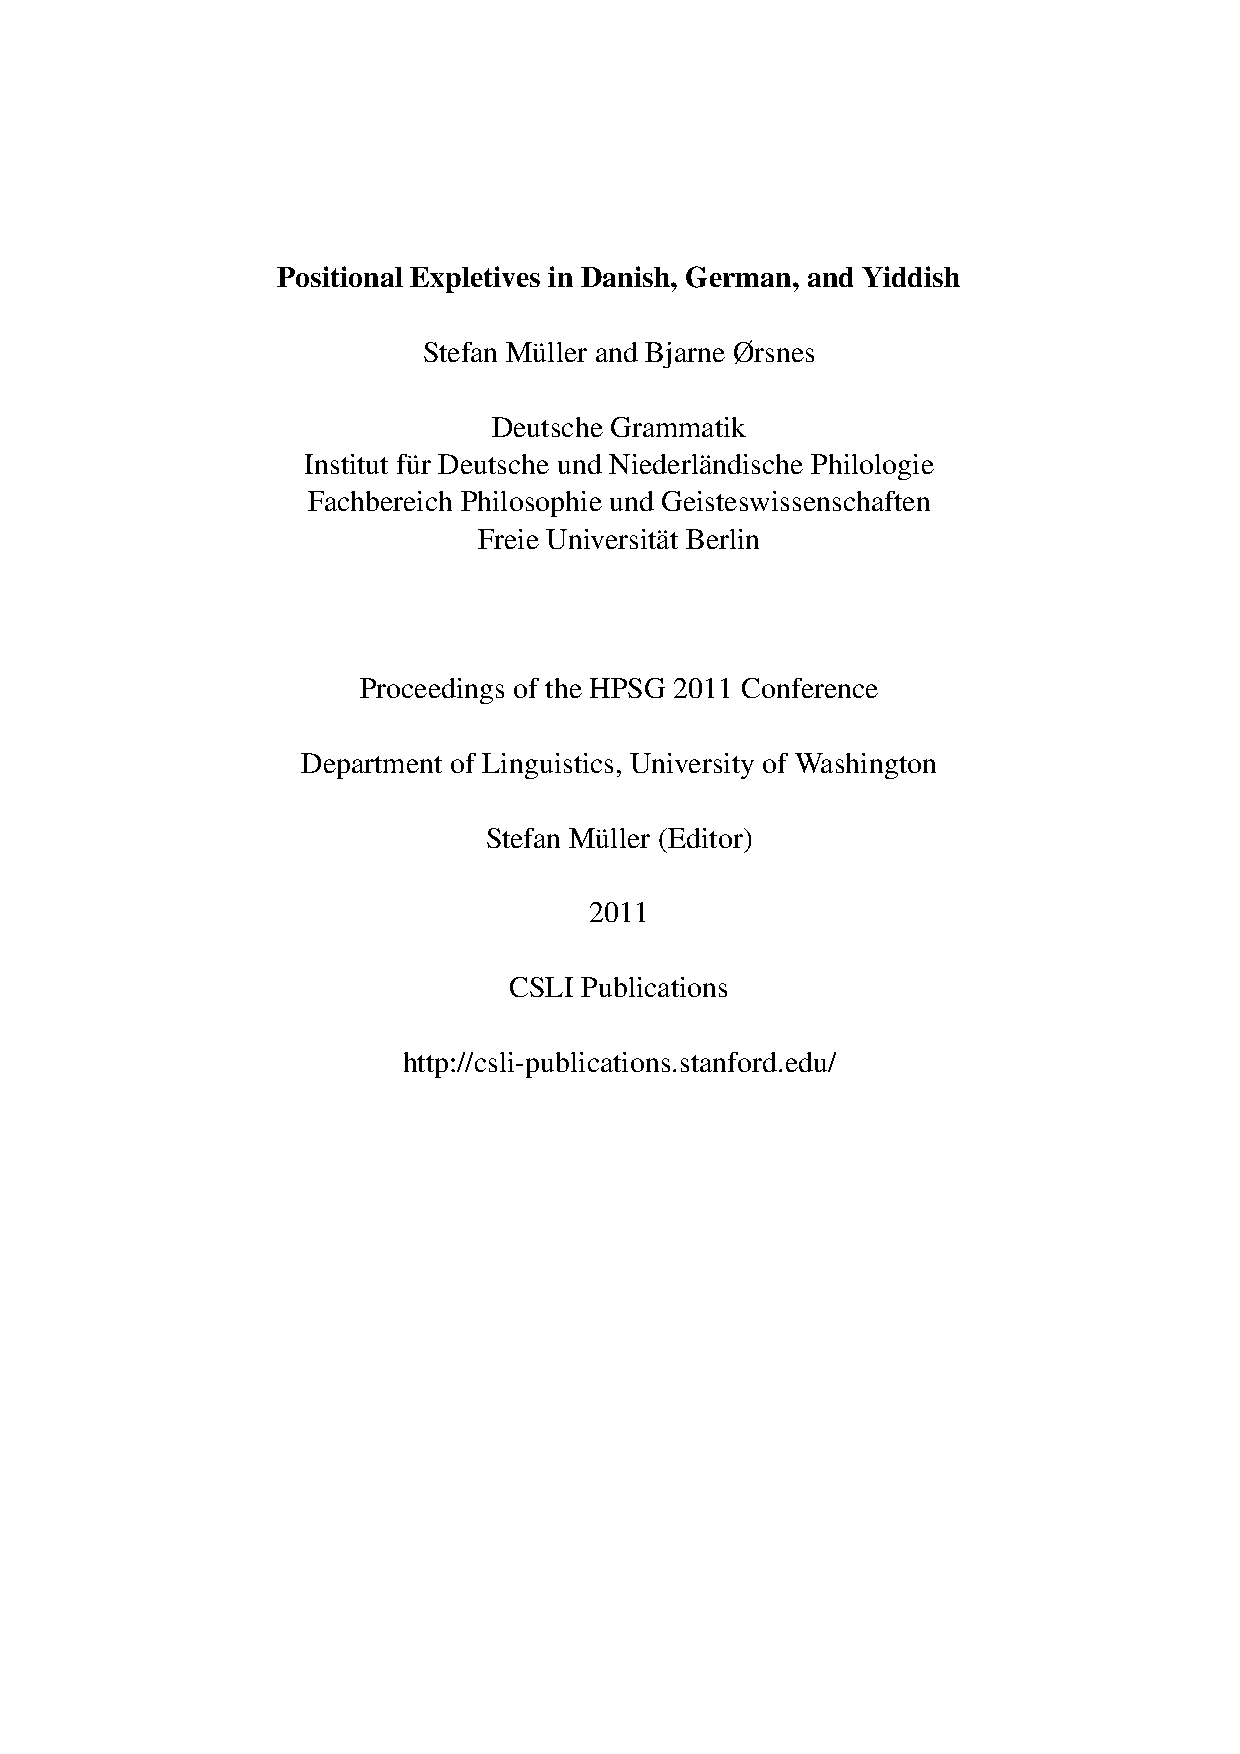
\includepdf[pages=-,pagecommand=\thispagestyle{plain},
            addtotoc={1,section,1,
            {Stefan Müller and Bjarne Ørsnes: Positional Expletives in Danish, German, and Yiddish},
             moe}]{mueller-oersnes.pdf}

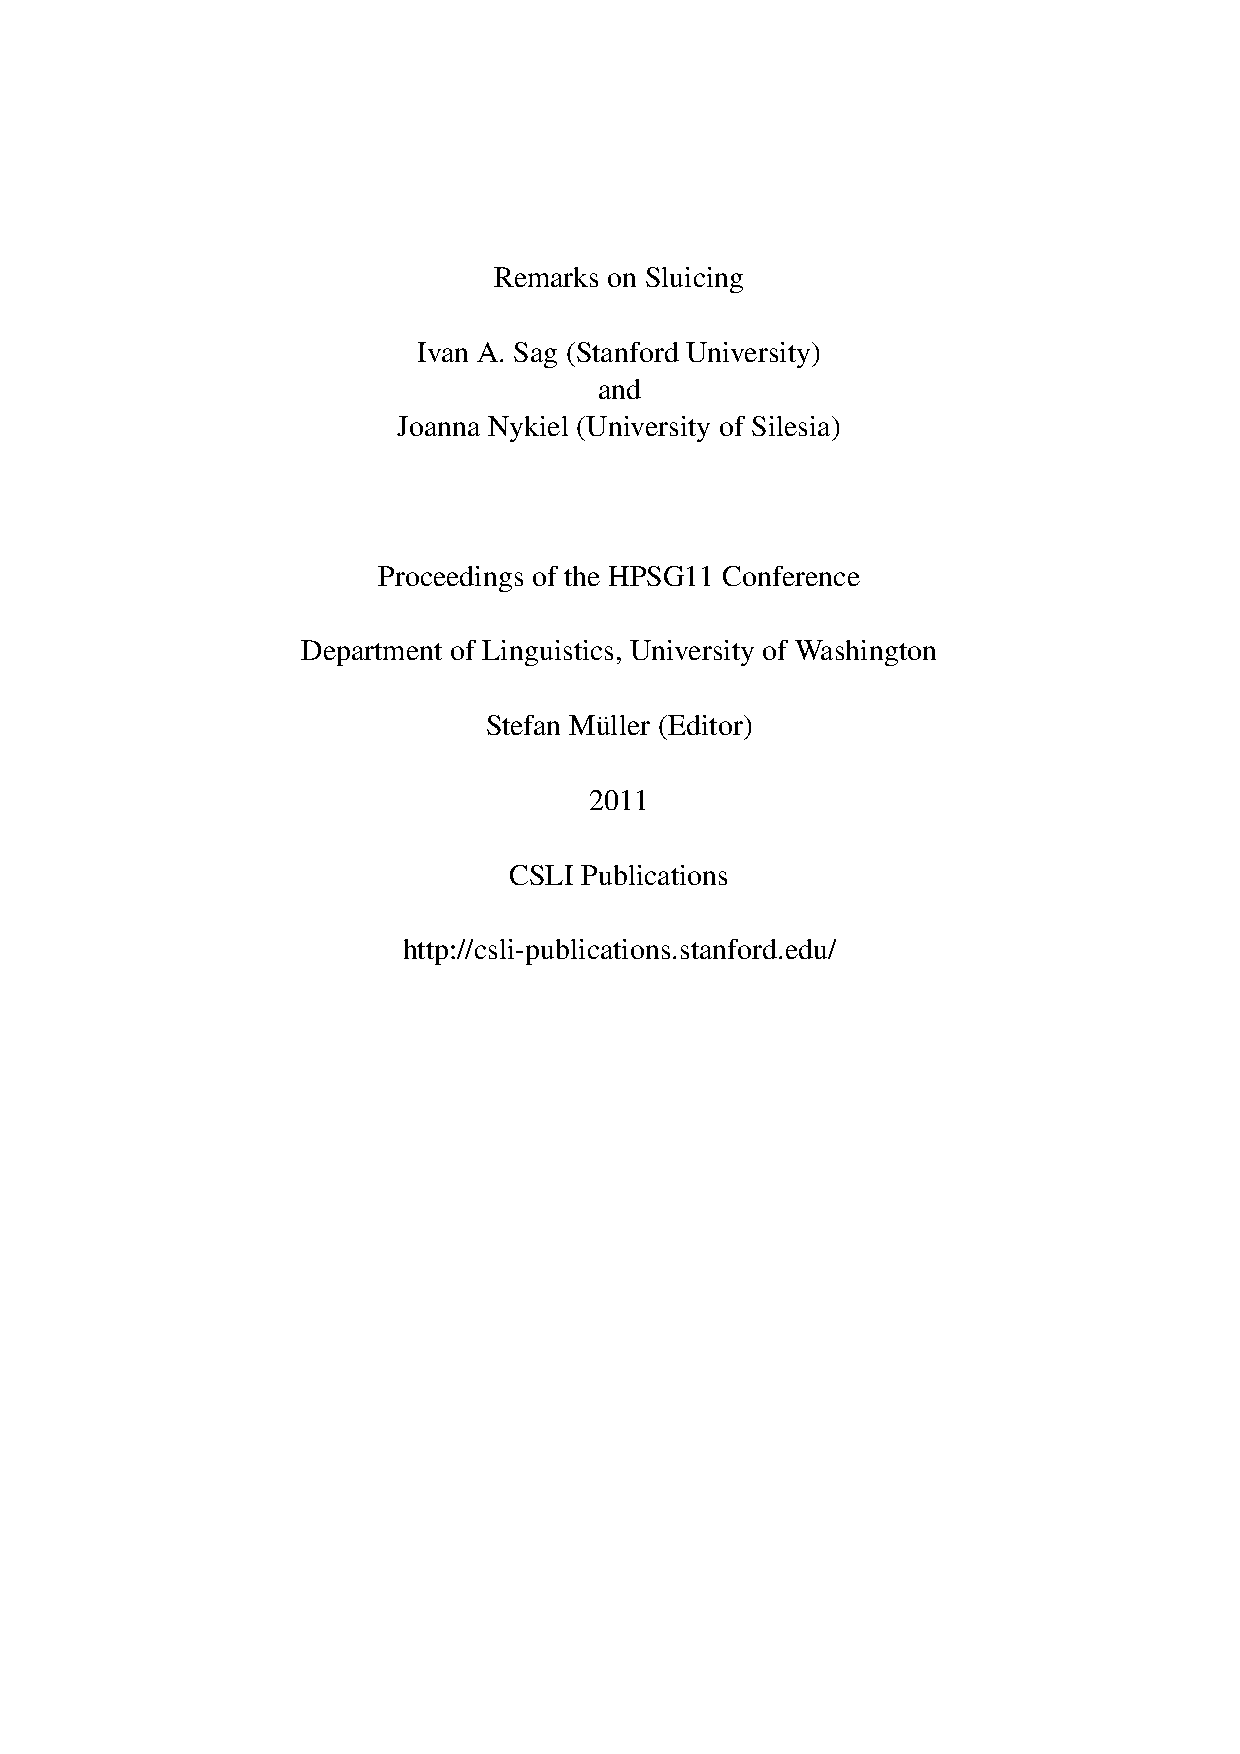
\includepdf[pages=-,pagecommand=\thispagestyle{plain},
            addtotoc={1,section,1,
            {Ivan A. Sag and Joanna Nykiel: Remarks on Sluicing},
             sn}]{sag-nykiel.pdf}


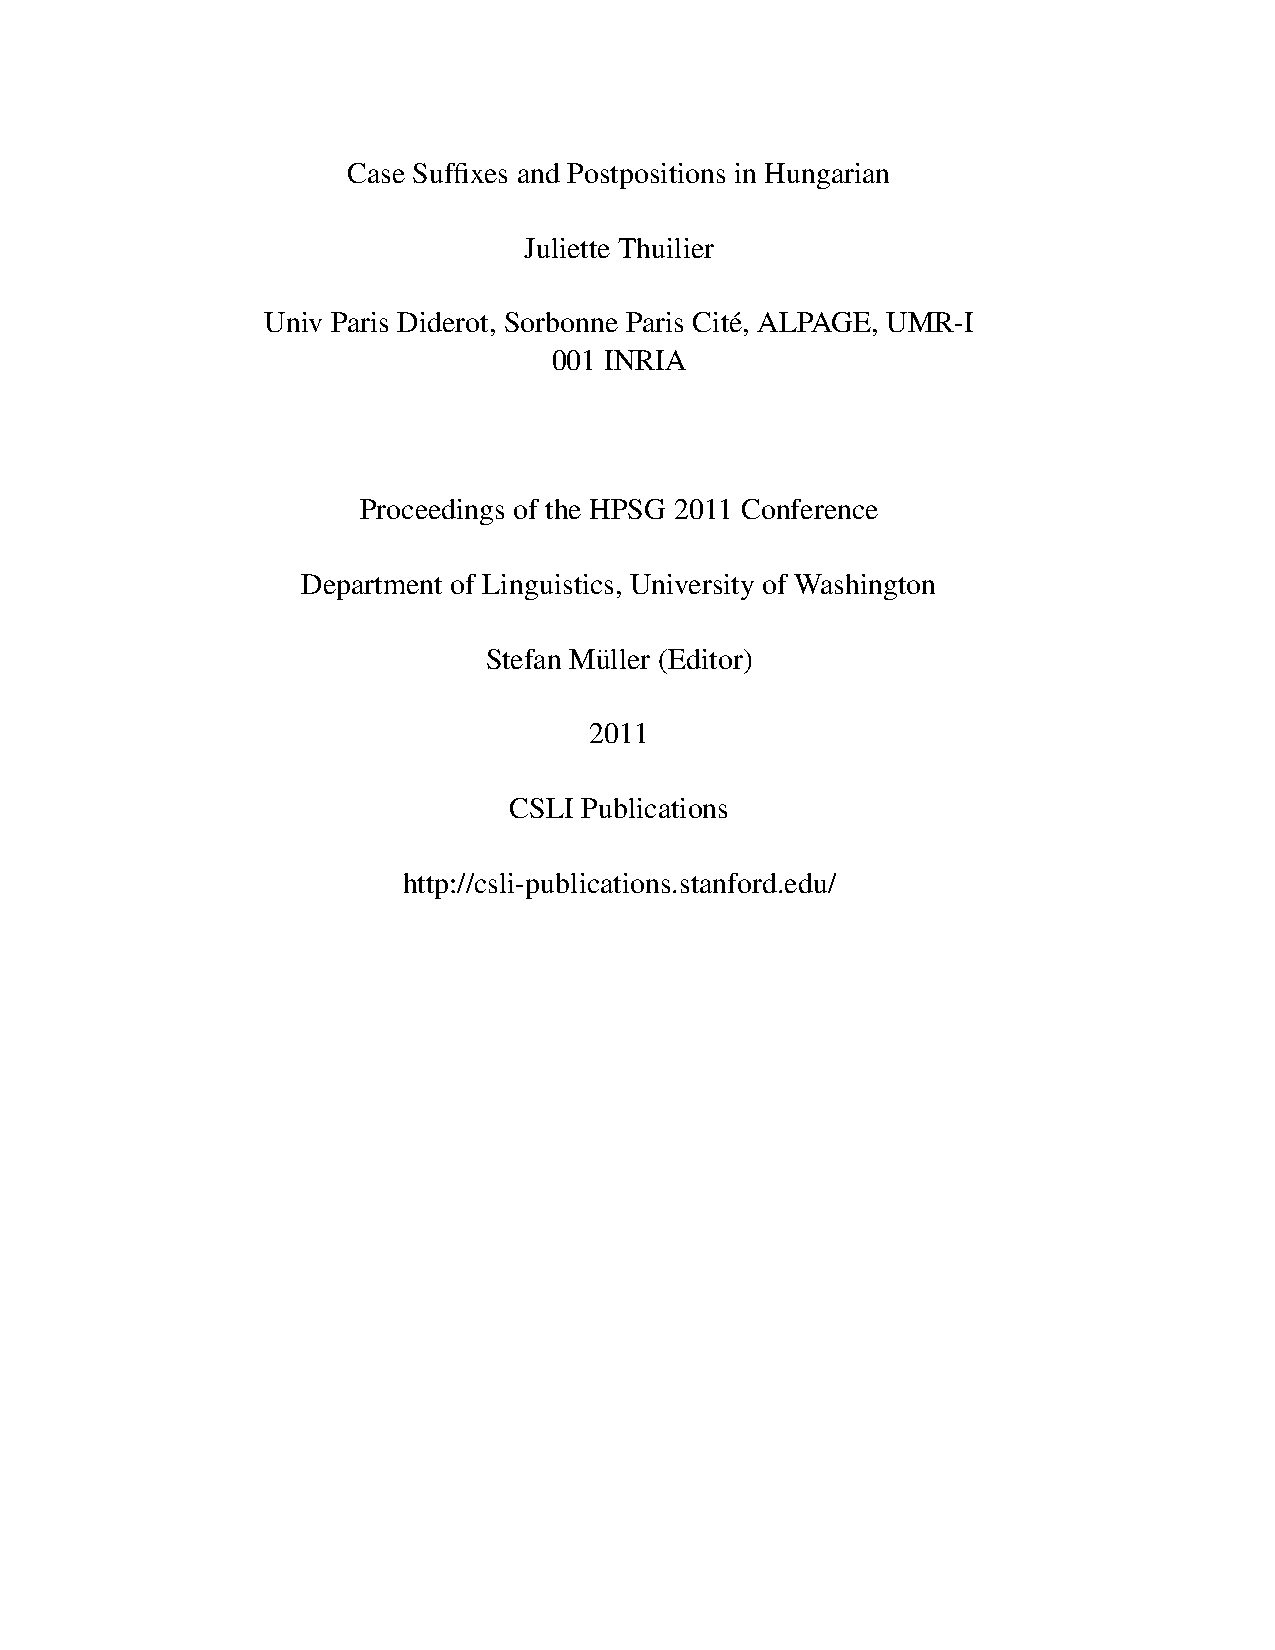
\includepdf[pages=-,pagecommand=\thispagestyle{plain},
            addtotoc={1,section,1,
            {Juliette Thuilier: Case Suffixes and Postpositions in Hungarian},
             thuilier}]{thuilier.pdf}

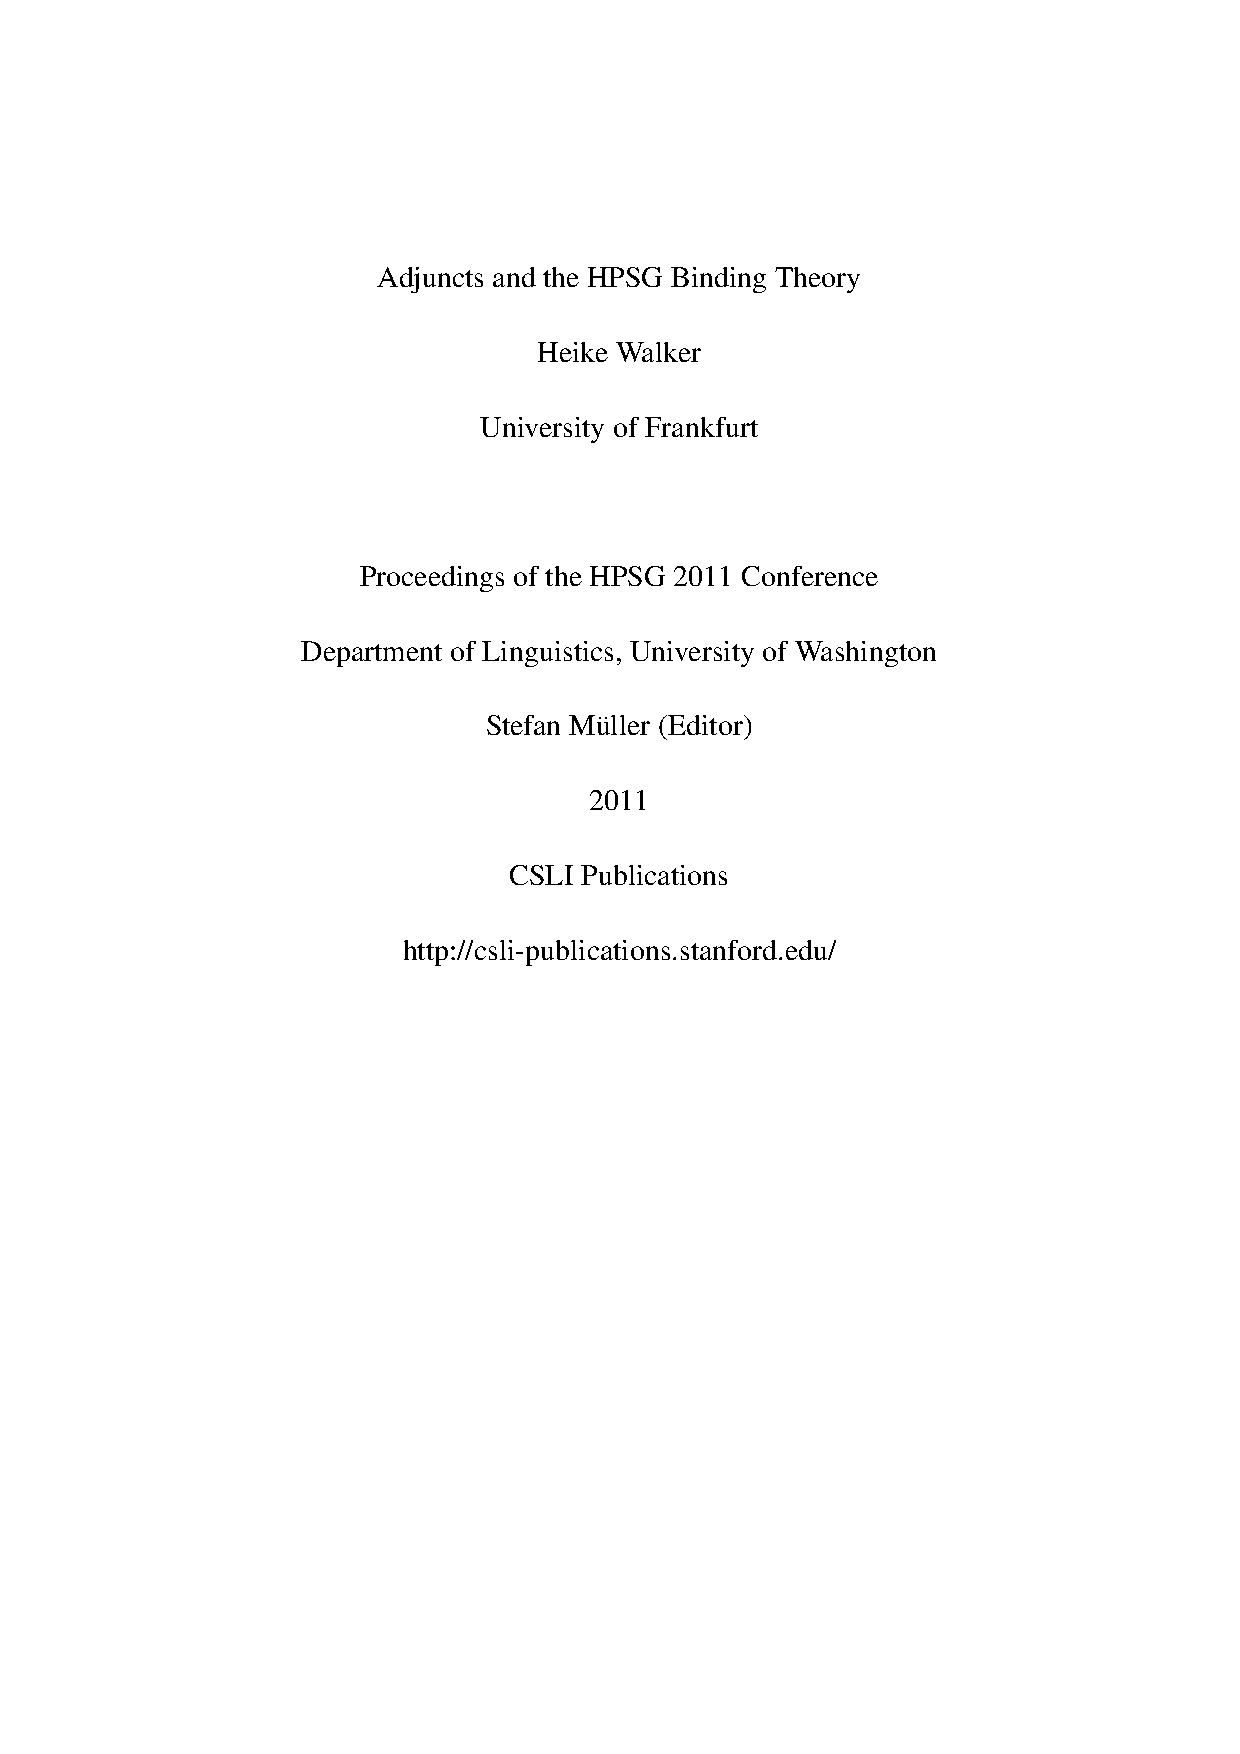
\includepdf[pages=-,pagecommand=\thispagestyle{plain},
            addtotoc={1,section,1,
            {Heike Walker: Adjuncts and the HPSG Binding Theory},
             walker}]{walker.pdf}


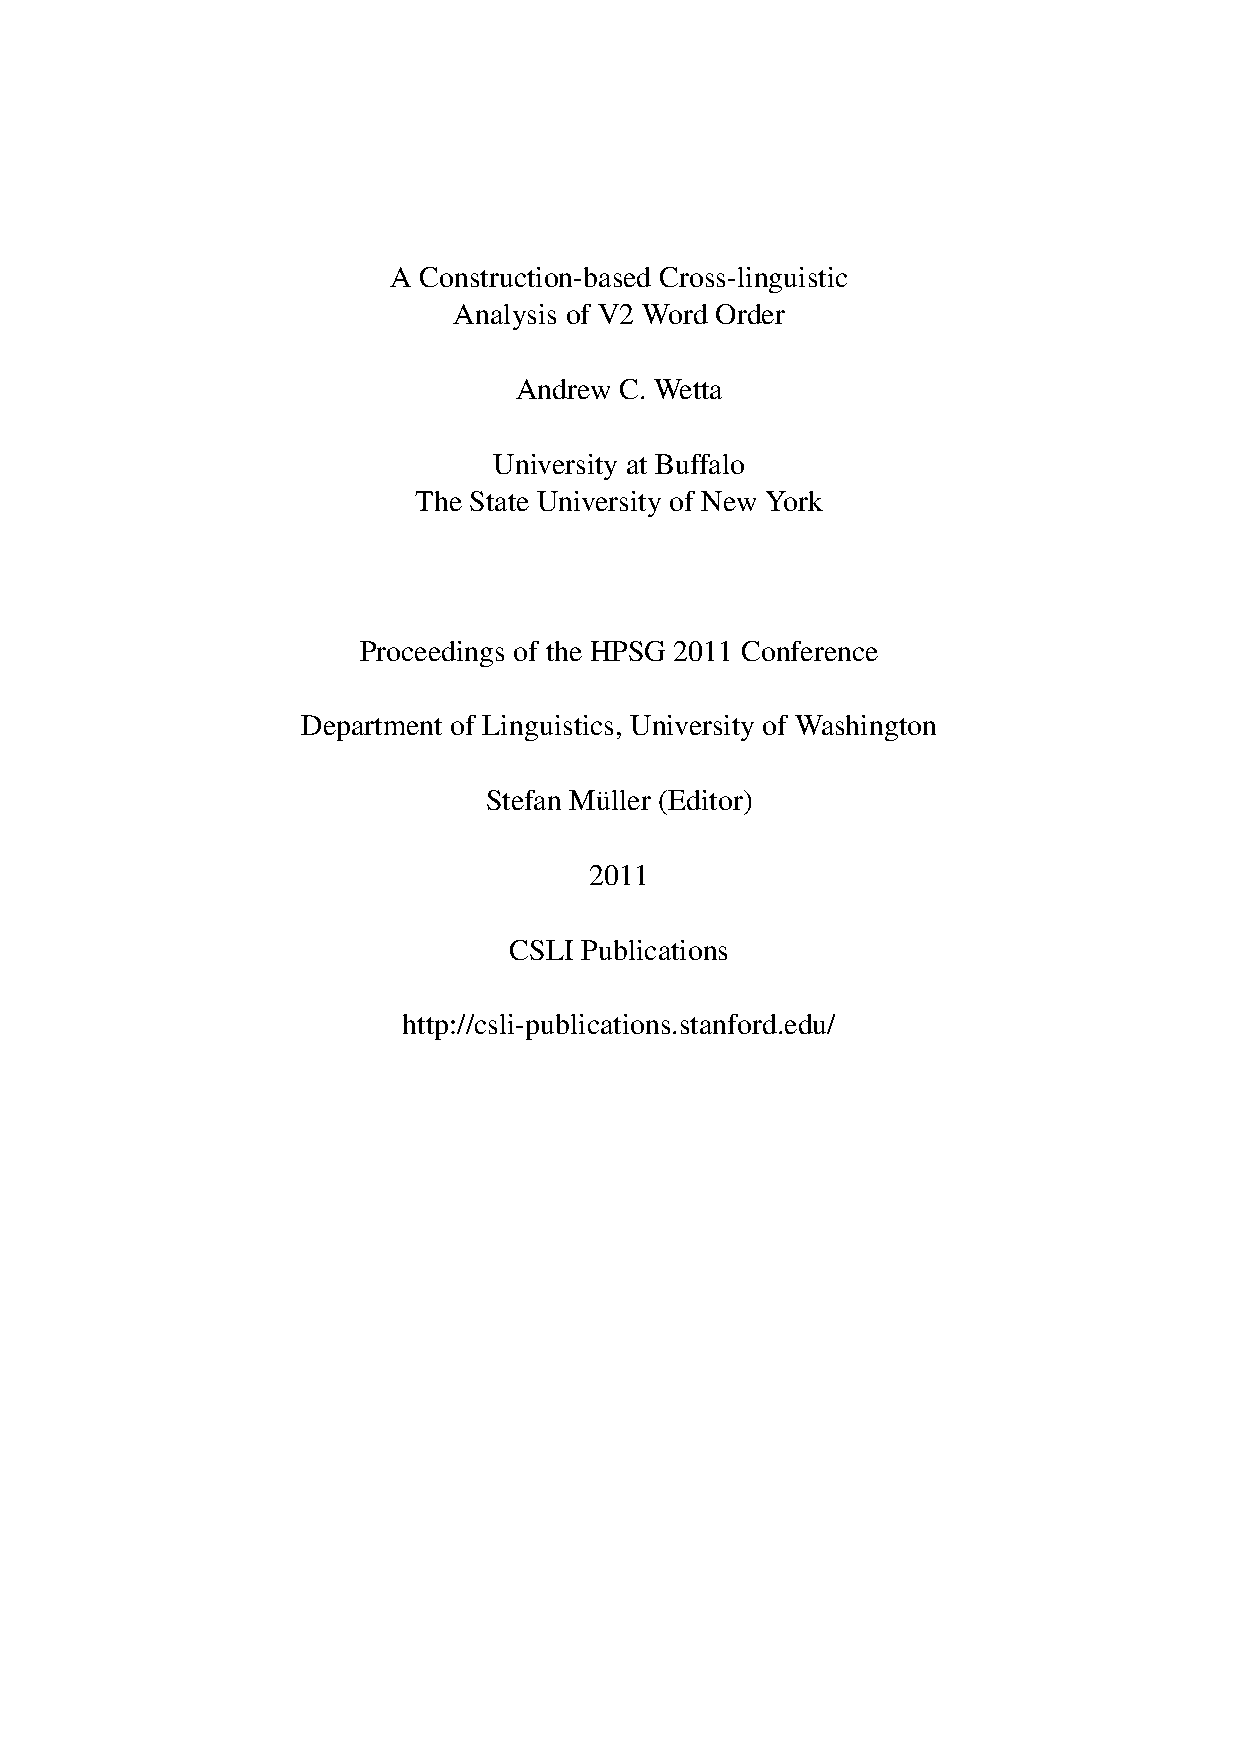
\includepdf[pages=-,pagecommand=\thispagestyle{plain},
            addtotoc={1,section,1,
            {Andrew C. Wetta: A Construction-based Cross-linguistic Analysis of V2 Word Order},
             wetta}]{wetta.pdf}


\part{Contributions to the Workshop on Information Structure and Formal Grammar}


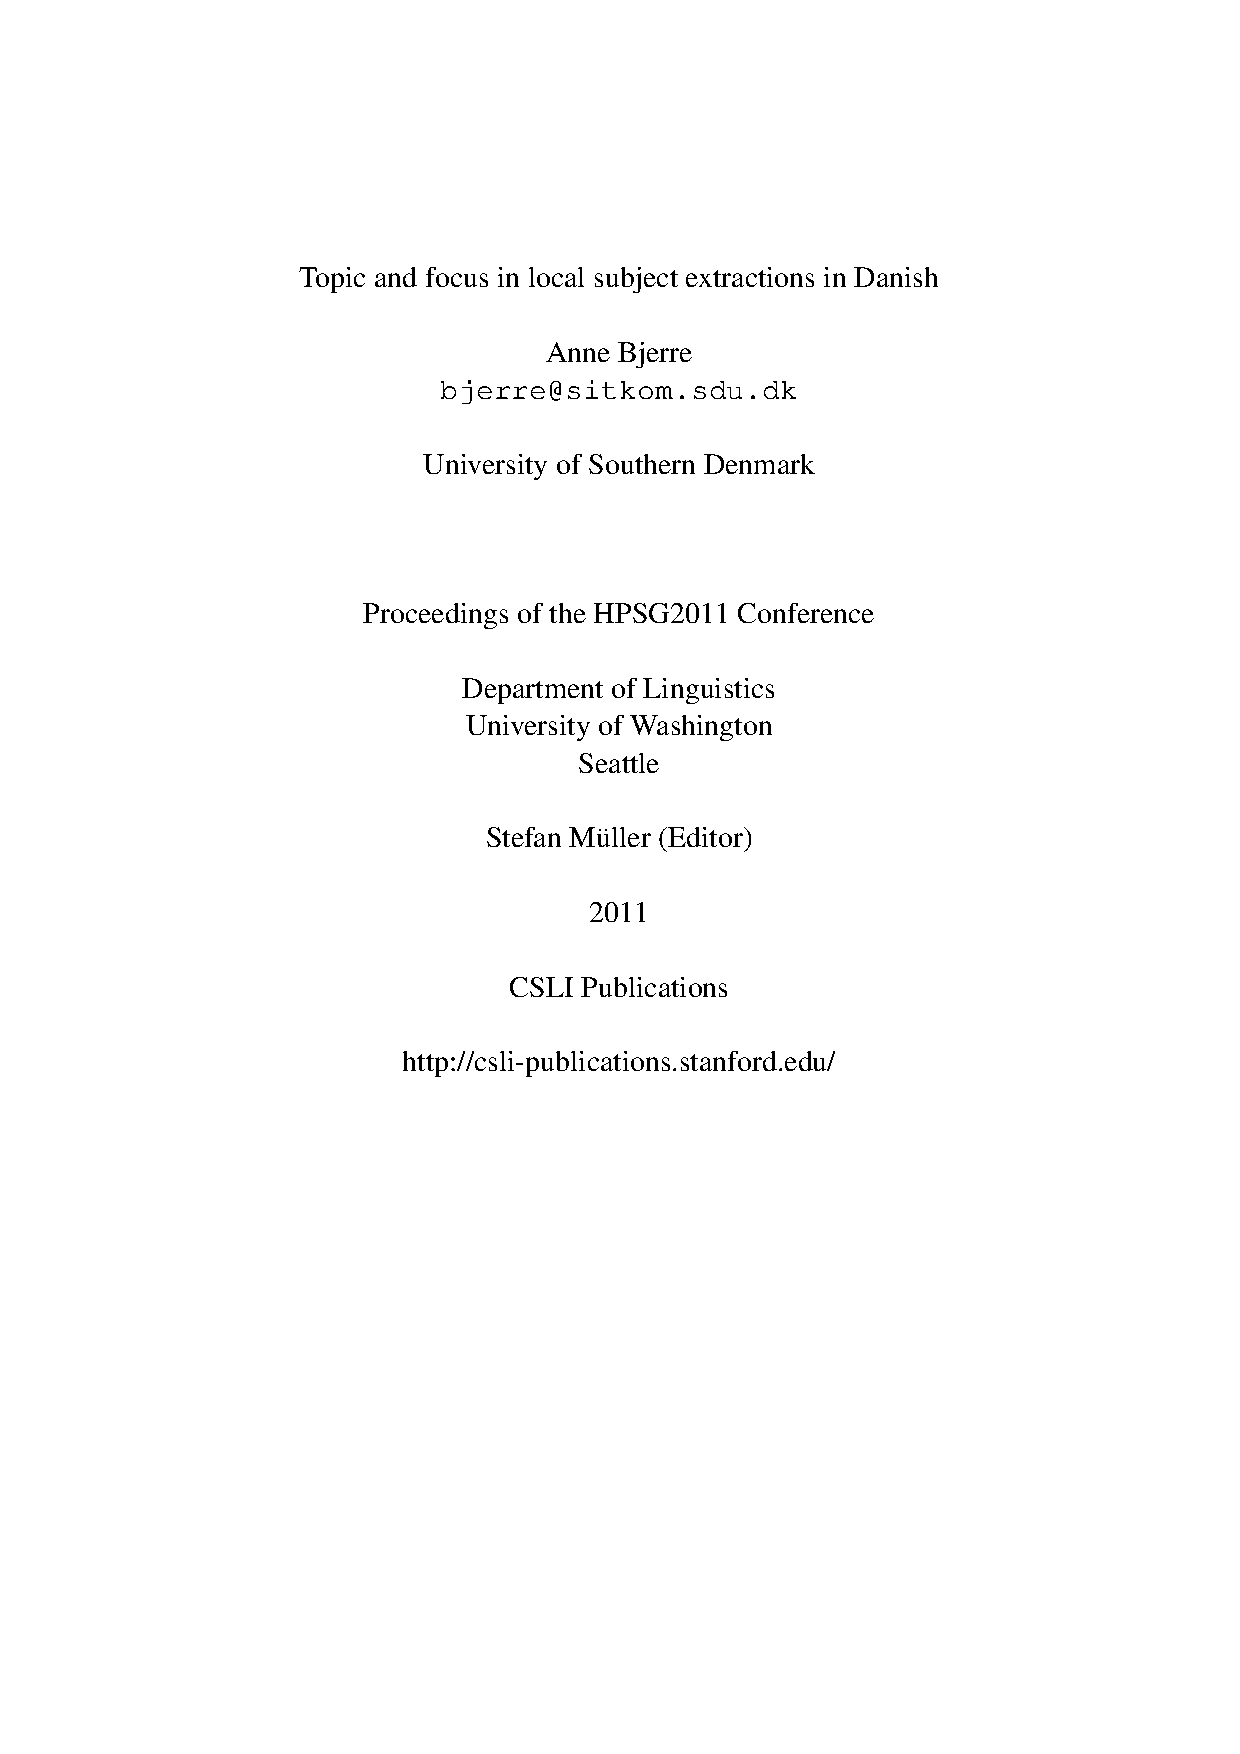
\includepdf[pages=-,pagecommand=\thispagestyle{plain},
            addtotoc={1,section,1,
            {Anne Bjerre: Topic and focus in local subject extractions in Danish},
             bjerre}]{bjerre.pdf}

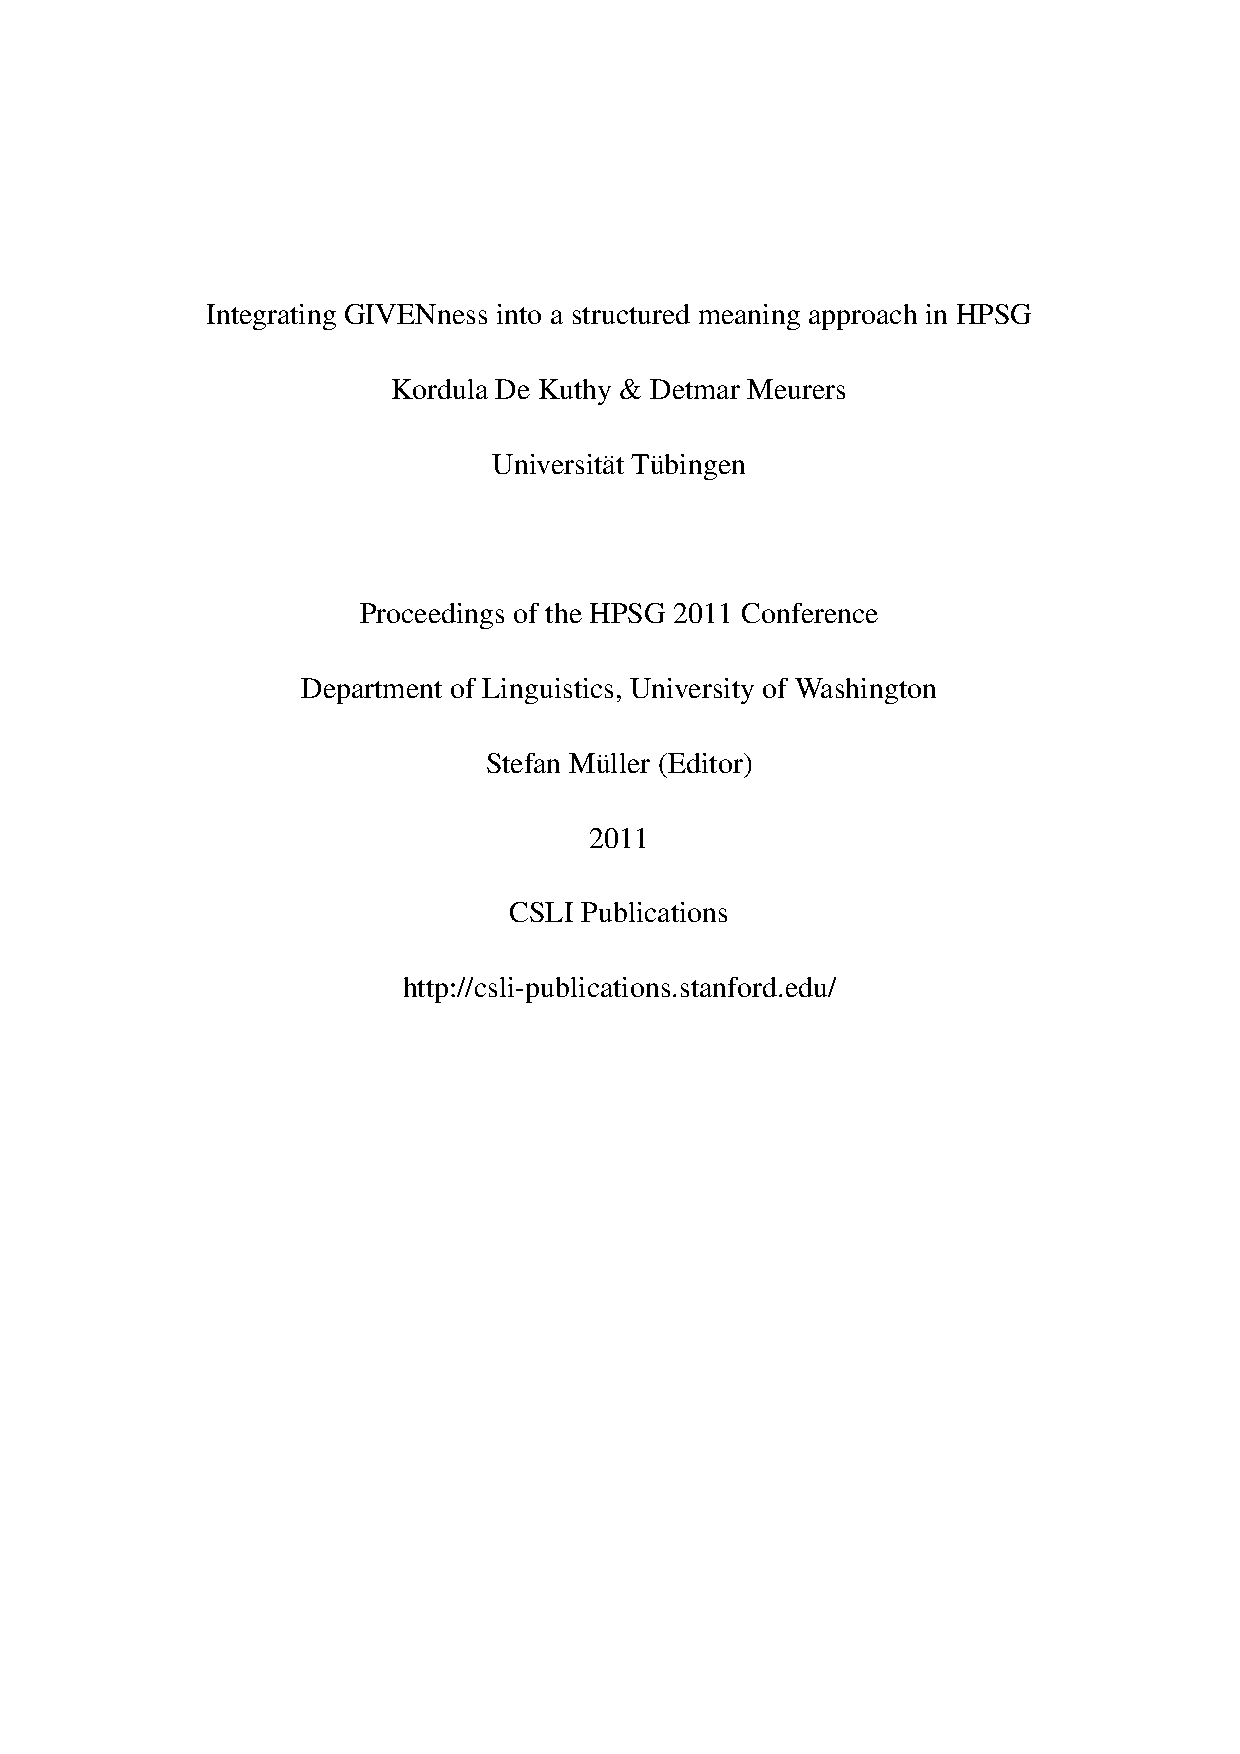
\includepdf[pages=-,pagecommand=\thispagestyle{plain},
            addtotoc={1,section,1,
            {Kordula De Kuthy and Detmar Meurers: Integrating GIVENness into a structured meaning approach in HPSG},
             dkm}]{dekuthy-meurers.pdf}

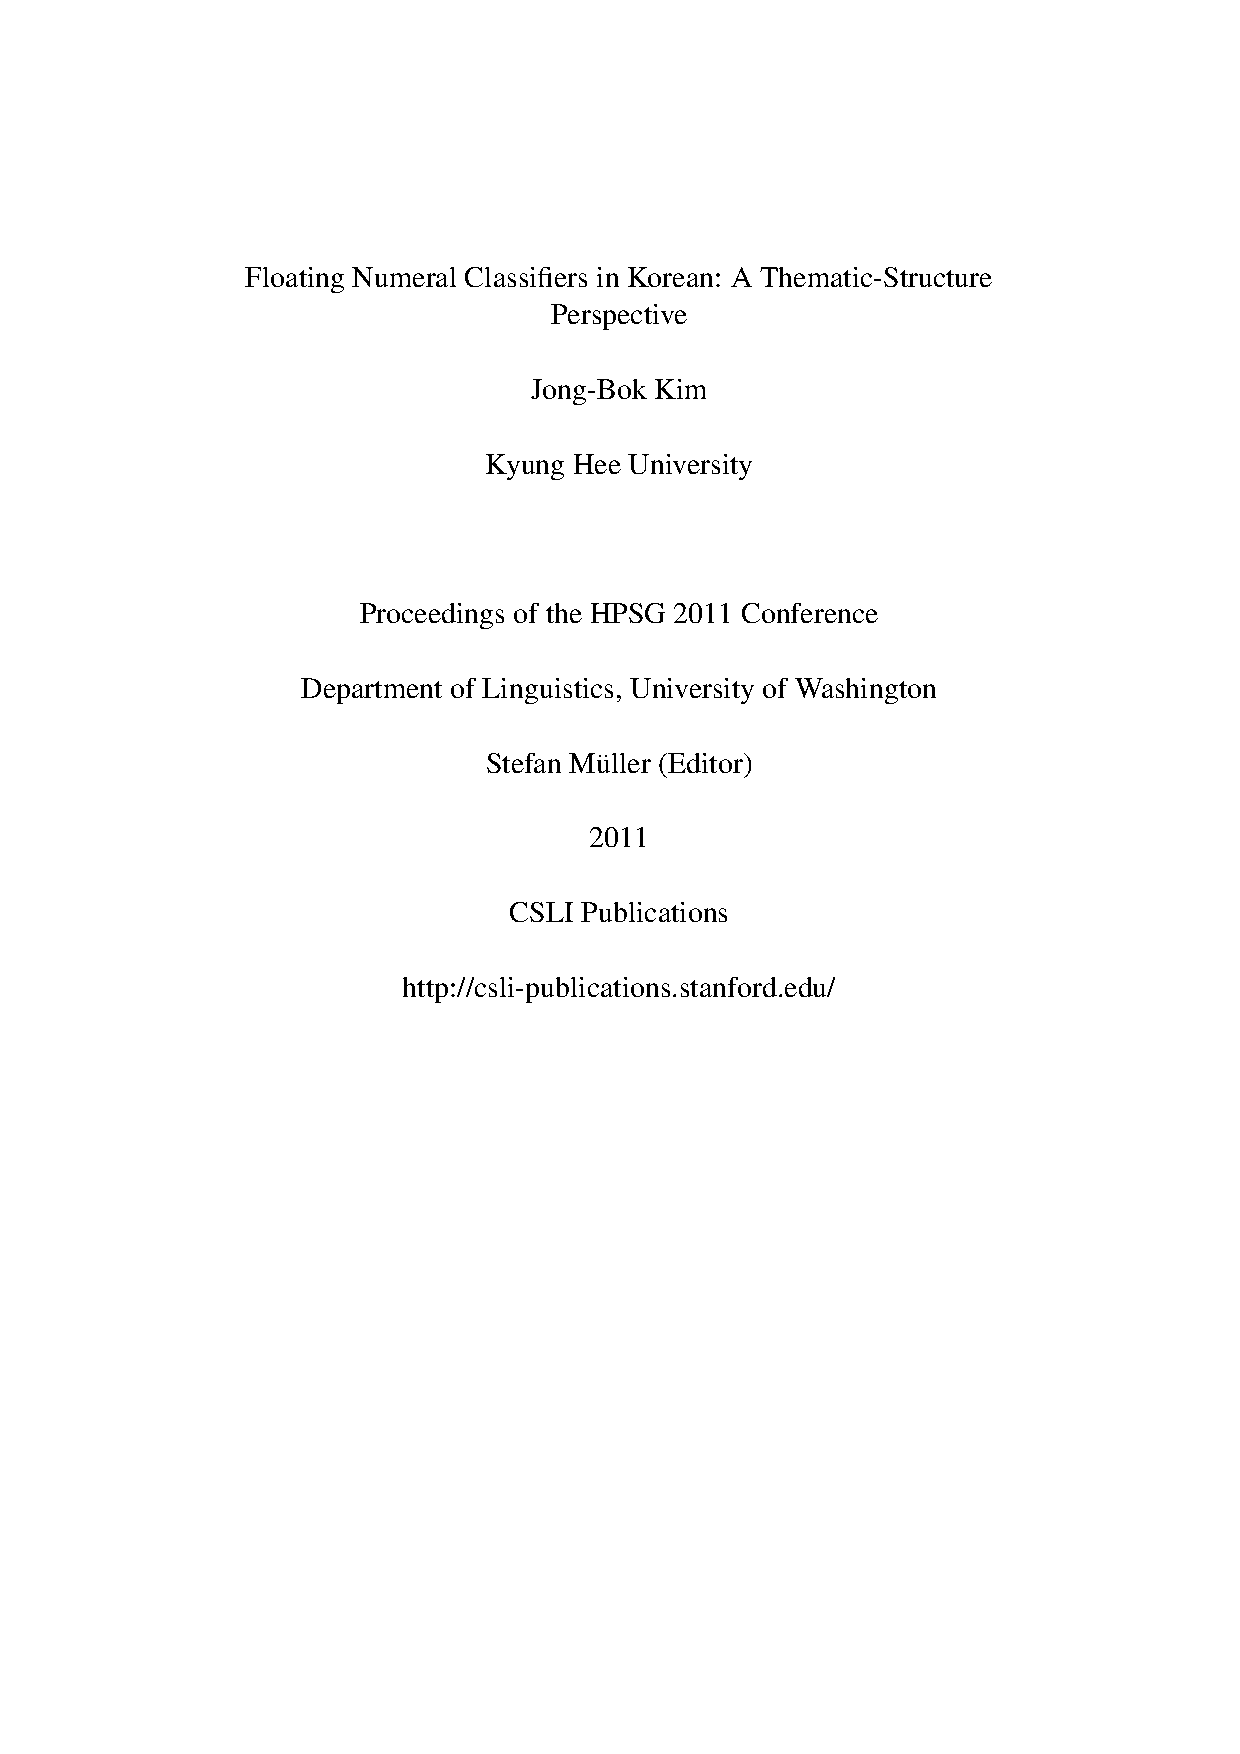
\includepdf[pages=-,pagecommand=\thispagestyle{plain},
            addtotoc={1,section,1,
            {Jong-Bok Kim: Floating Numeral Classifiers in Korean: A Thematic-Structure Perspective},
             kim}]{kim.pdf}

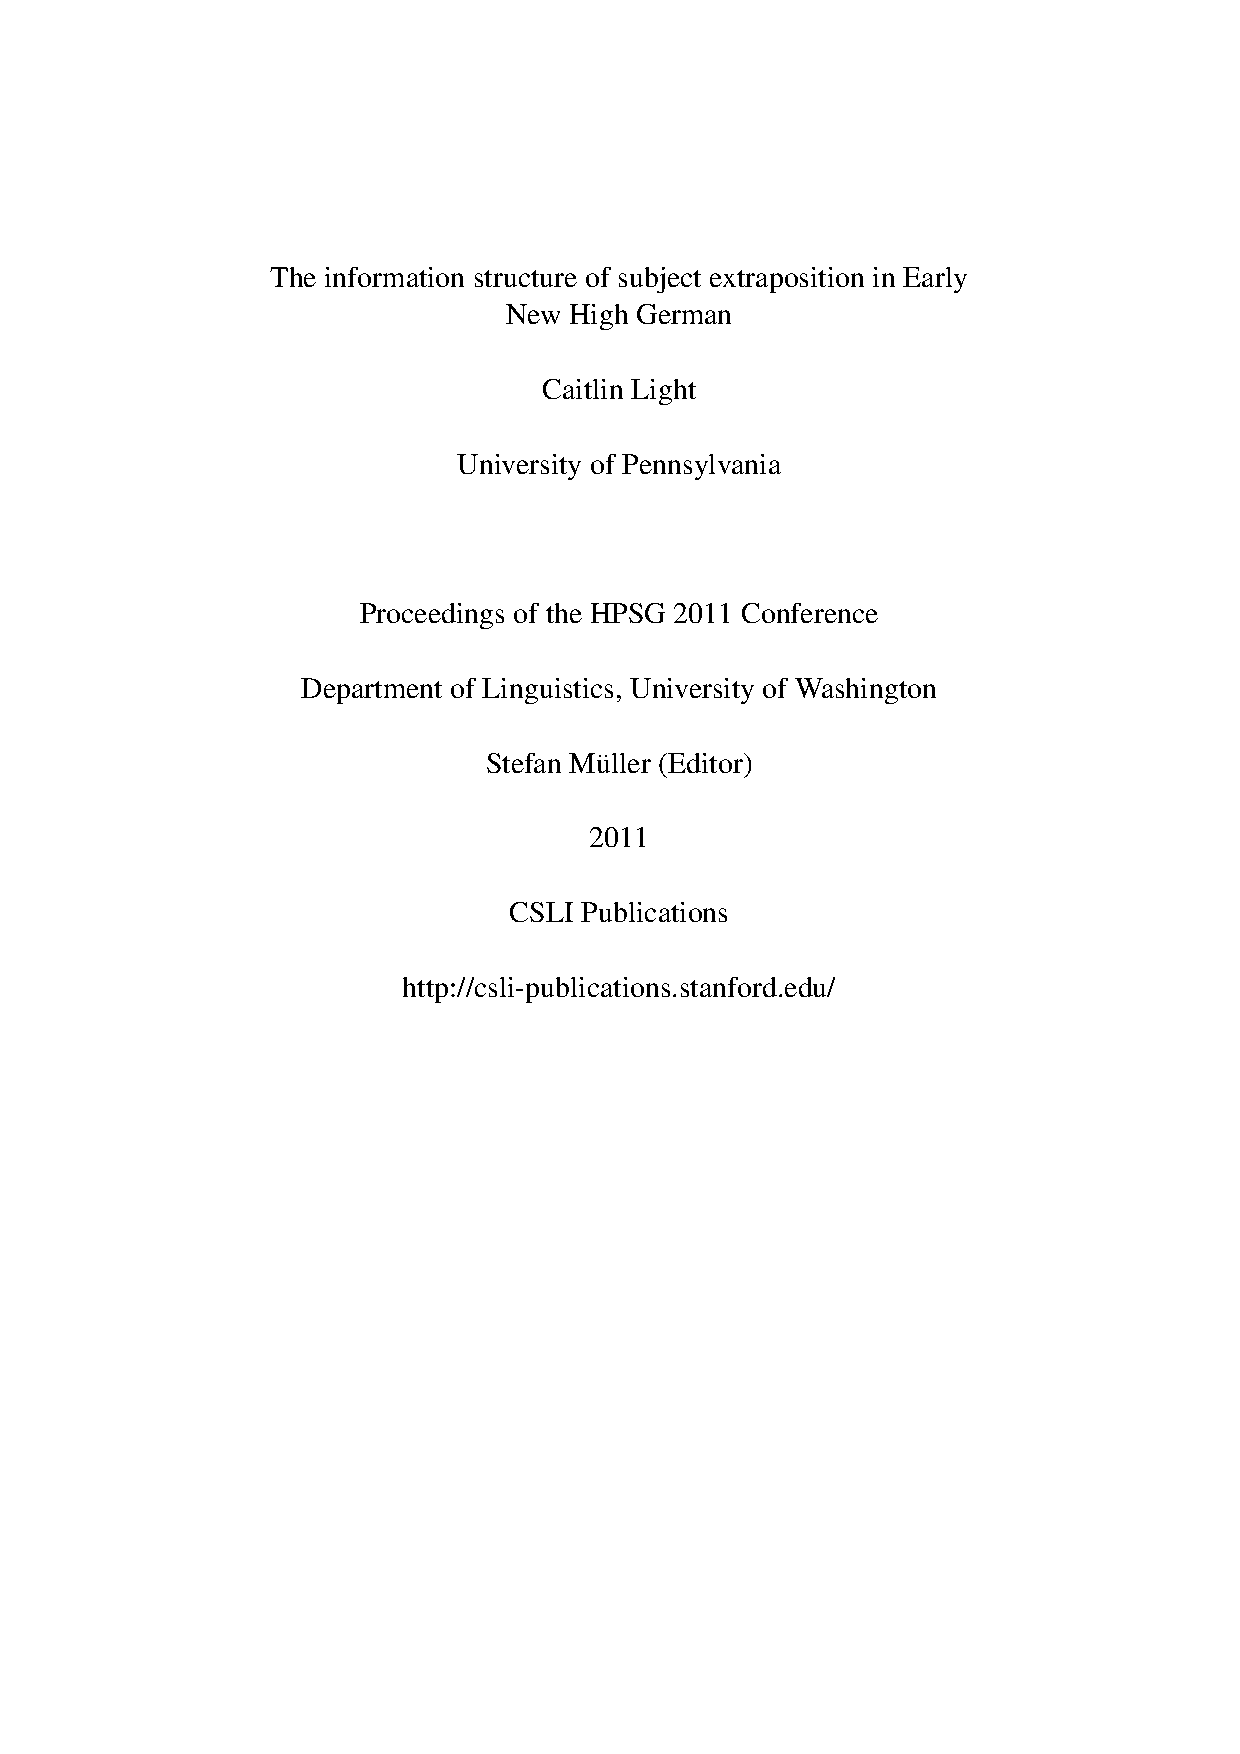
\includepdf[pages=-,pagecommand=\thispagestyle{plain},
            addtotoc={1,section,1,
            {Caitlin Light: The information structure of subject extraposition in Early New High German},
             light}]{light.pdf}

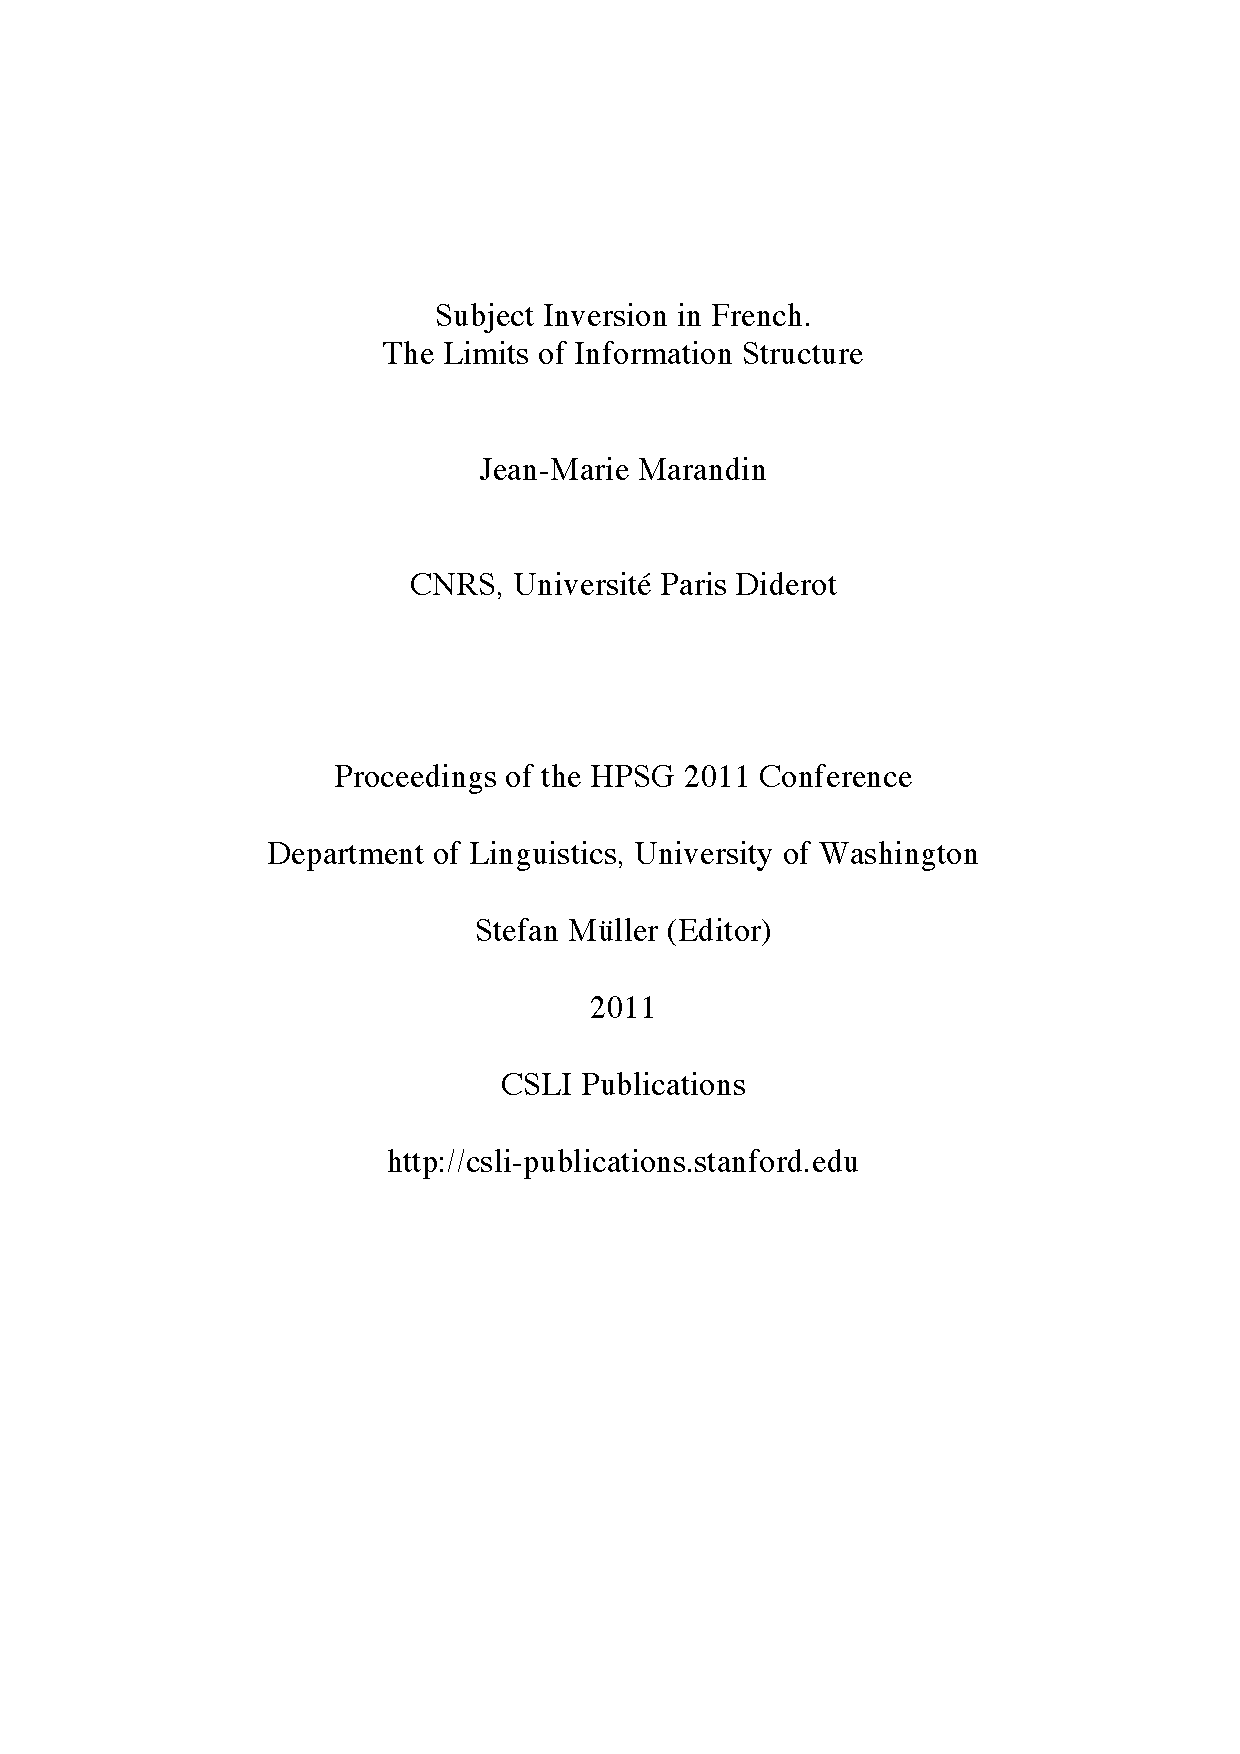
\includepdf[pages=-,pagecommand=\thispagestyle{plain},
            addtotoc={1,section,1,
            {Jean-Marie Marandin: Subject Inversion in French. The Limits of Information Structure},
             marandin}]{marandin.pdf}


\includepdf[pages=-,pagecommand=\thispagestyle{plain},
            addtotoc={1,section,1,
            {Sanghoun Song and Emily M. Bender: Using Information Structure to Improve Transfer-based MT},
             sb}]{song-bender.pdf}

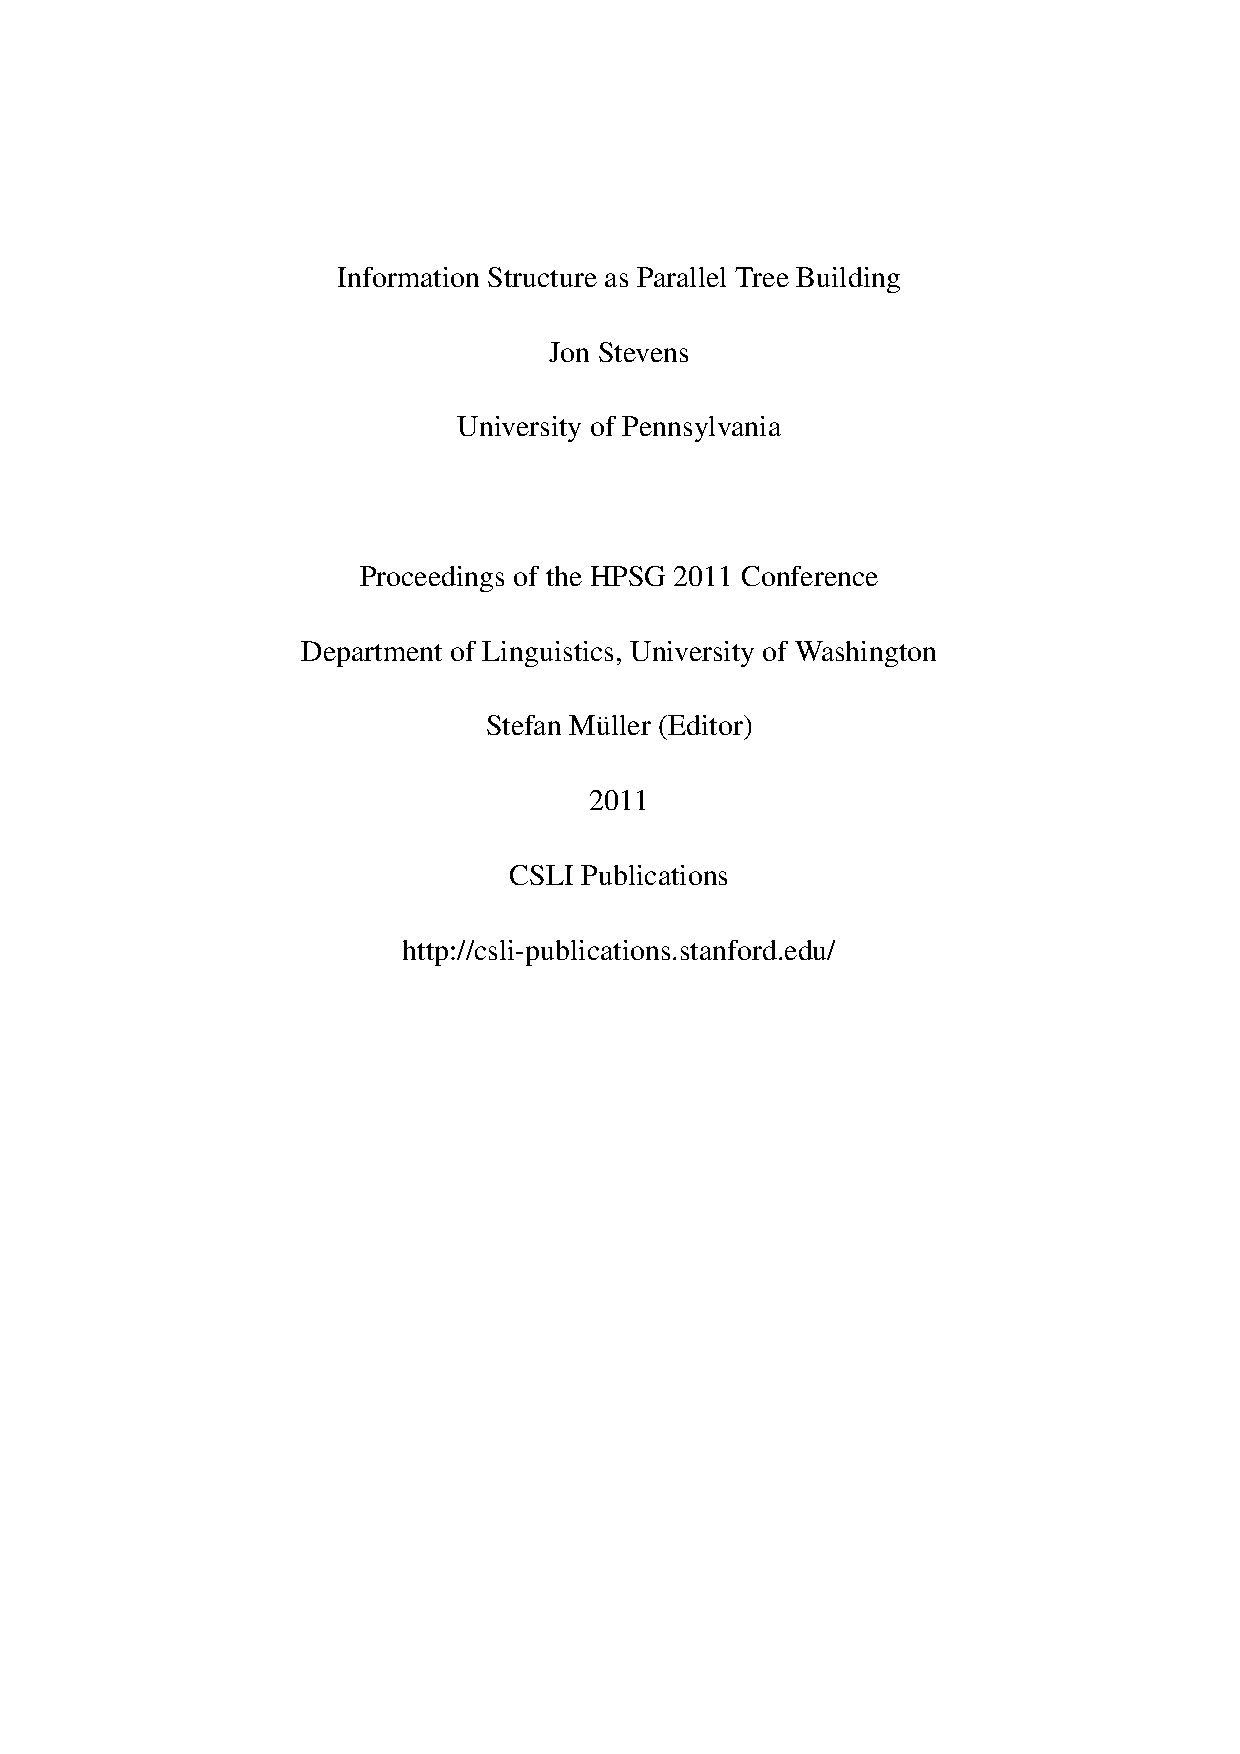
\includepdf[pages=-,pagecommand=\thispagestyle{plain},
            addtotoc={1,section,1,
            {Jon Stevens: Information Structure as Parallel Tree Building},
             stevens}]{stevens.pdf}



\end{document}

